\chapter{Inference from the 21cm signal}

\begin{bf}
  \author{Bradley Greig}\\
  
Abstract\\
\end{bf}

In the previous chapters we have discussed in-depth the astrophysical and cosmological information that is encoded by the cosmic 21-cm signal. However, once we have a measurement, how do we extract this information from the signal? This chapter focusses on the inference of the interesting astrophysics and cosmology once we obtain a detection of the 21-cm signal. 

Essentially, inference of the astrophysics can be broken down into three parts:
\begin{itemize}
\item[1.] \textbf{Compression of the observed data into a manageable dataset:} The observed 21-cm signal varies spatially as well as along the line-of-sight (frequency or redshift dimension) to provide a full three dimensional movie of the intergalactic medium in the early Universe. However, the signal is faint, requiring either statistical methods to sum the data in order to increase the signal-to-noise or sophisticated approaches to extract the faint signal directly. 
\item[2.] \textbf{An efficient method to model/simulate the 21-cm signal:} In order to interpret the observations and understand the astrophysical processes responsible, we must be able to produce physically motivated models capable of replicating the signal. Further, these must be as computationally efficient as possible in order to be able to realistically investigate the 21-cm signal.
\item[3.] \textbf{A robust probabilistic framework to extract the physics:} The observed 21-cm signal is dependent on numerous physical processes, which within our models or simulations are described by many unknown parameters. Further, these contain approximations in order to deal with the requisite dynamic range. We must be able to characterise our ignorance in a meaningful way in order to be truly able to infer the astrophysical processes of the epoch of reionisation and cosmic dawn.
\end{itemize}
\noindent
In this chapter we will focus on each separately, discussing the current state-of-the-art in inferring the 21cm signal.

\section{What do we actually measure?}

The 21-cm signal from the neutral hydrogen in the intergalactic medium is measured by its brightness temperature, $T_{\rm b}$. However, this cannot be measured directly, instead it is expressed as a brightness temperature contrast, $\delta T_{b}$, relative to the Cosmic Microwave Background (CMB) temperature, $T_{\rm CMB}$ \cite{Furlanetto:2006}: 
\begin{equation} \label{eq:delTb}
\delta T_{b}(\mathbf{x},\nu) \equiv T_{\rm b}(\mathbf{x},\nu) - T_{\rm CMB, 0}.
\end{equation}
As such, this brightness temperature contrast can be seen either in emission or absorption, dependent on the 21-cm brightness temperature which itself is dependent on the excitation state of the neutral hydrogen (i.e. its spin temperature, $T_{\rm S}$, see {\color{red} previous chapter}). We can re-express Equation~\ref{eq:delTb} in terms of $T_{\rm S}$ to recover {\color{red} (should have been introduced in a previous chapter)},
\begin{equation} \label{eq:delTb_Ts}
\delta T_{b}(\mathbf{x},\nu) \equiv \frac{T_{\rm S}(\mathbf{x},\nu) - T_{\rm CMB}(z)}{1+z} \left( 1 - {\rm e}^{-\tau_{\nu_{0}}(\mathbf{x},\nu) } \right),
\end{equation}
where $\tau_{\nu_{0}}$ is the optical depth of the 21-cm line. $\delta T_{b}(\mathbf{x},\nu)$ varies spatially due to its two-dimensional angular position on the sky while it varies along the line-of-sight direction owing to the 21-cm line being redshifted by cosmological expansion (i.e. adding a frequency or time dependence to the signal). Thus, measuring $\delta T_{b}(\mathbf{x},\nu)$ can reveal a full three-dimensional movie of the neutral hydrogen in the early Universe.

Unfortunately, $\delta T_{b}(\mathbf{x},\nu)$ is faint. Further, in reality it is buried under numerous astrophysical foregrounds all of which are orders of magnitude brighter {\color{red} (see relevant chapters for more detailed discussions)}. In order to deal with this faint signal coupled with the astrophysical foregrounds, typically we seek to compress the data to boost the signal-to-noise or specifically tailor methods to extract the faint signal. In this chapter, we will discuss the numerous methods proposed in order to tease out the faint astrophysical signal from the noise.

\section{Optimal methods for characterising the 21-cm signal}

The first step in our efforts to be able to infer information about the astrophysical processes responsible for reionisation and the cosmic dawn is to explore optimal methods to characterise the 21-cm signal. In this section, we summarise the wide variety of approaches considered in the literature, highlighting the leverage that each is able to provide with respect to the underlying astrophysical processes. Note that throughout this chapter, all investigations into detecting the 21-cm signal are generated theoretically, either analytically or numerically. Thus, we urge the reader to refer to the citations in order to understand the limiting assumptions.

\subsection{Global signal} \label{sec:global}

The simplest way to deal with such a faint signal is to average it over as large a volume as possible. Since the 21-cm signal is visible across the entire sky, one can produce a complete sky-averaged (global) 21-cm brightness temperature as a function of frequency (redshift). Although the two-dimensional spatial information from the 21-cm signal is lost, the main advantage is that it is relatively cheap to observe, requiring comparatively simple instrumentation {\color{red} (see future chapter on global signal or observations?)}. A fact that several experiments have used in an attempt to provide a measurement of the 21-cm signal, given that a single radio dipole is capable of seeing essentially the entire sky at any one time. In Figure~\ref{fig:global}, we show a representative model of the global 21-cm signal, highlighting the major cosmological milestones that have been discussed in previous chapters. Thus, in each frequency bin, we measure an all-sky average of the 21-cm brightness temperature.

\begin{figure}[]
\begin{center}
%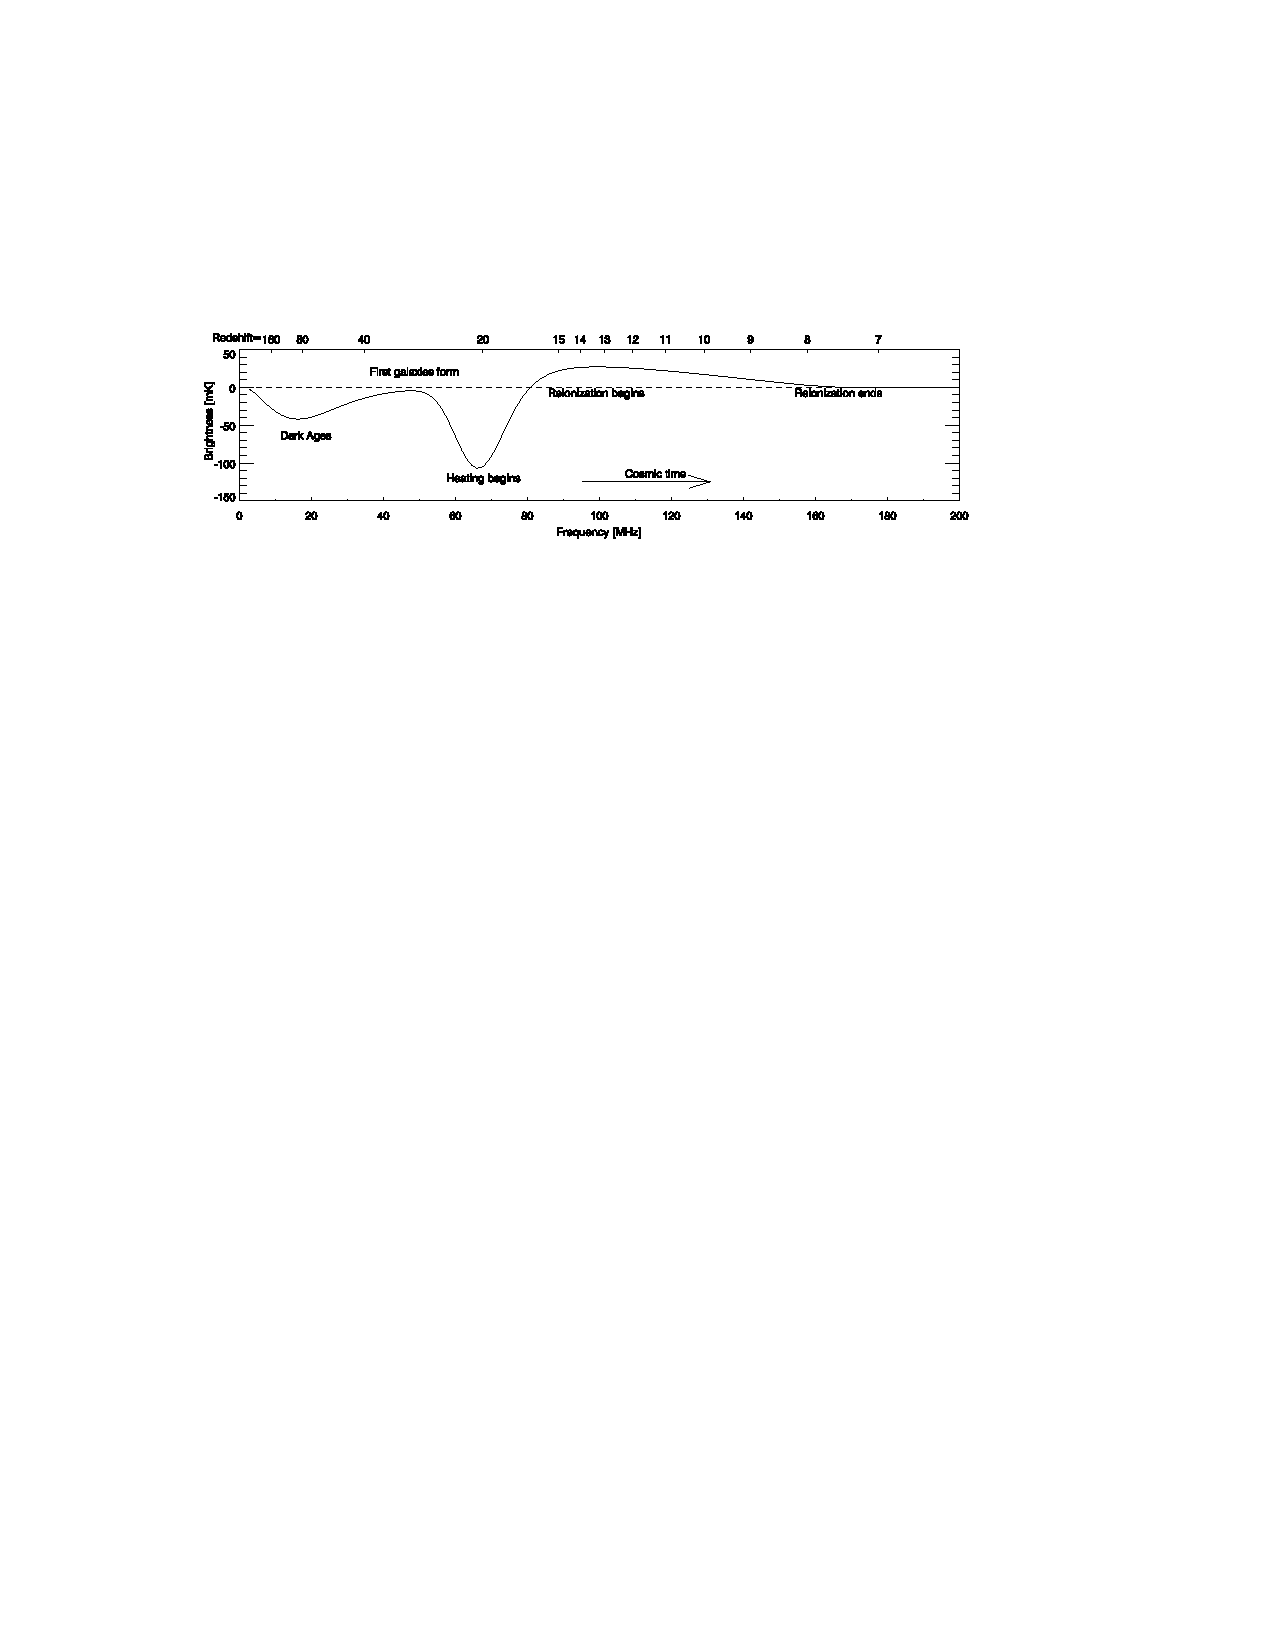
\includegraphics[width=1.\textwidth]{Greig/GlobalSignal}
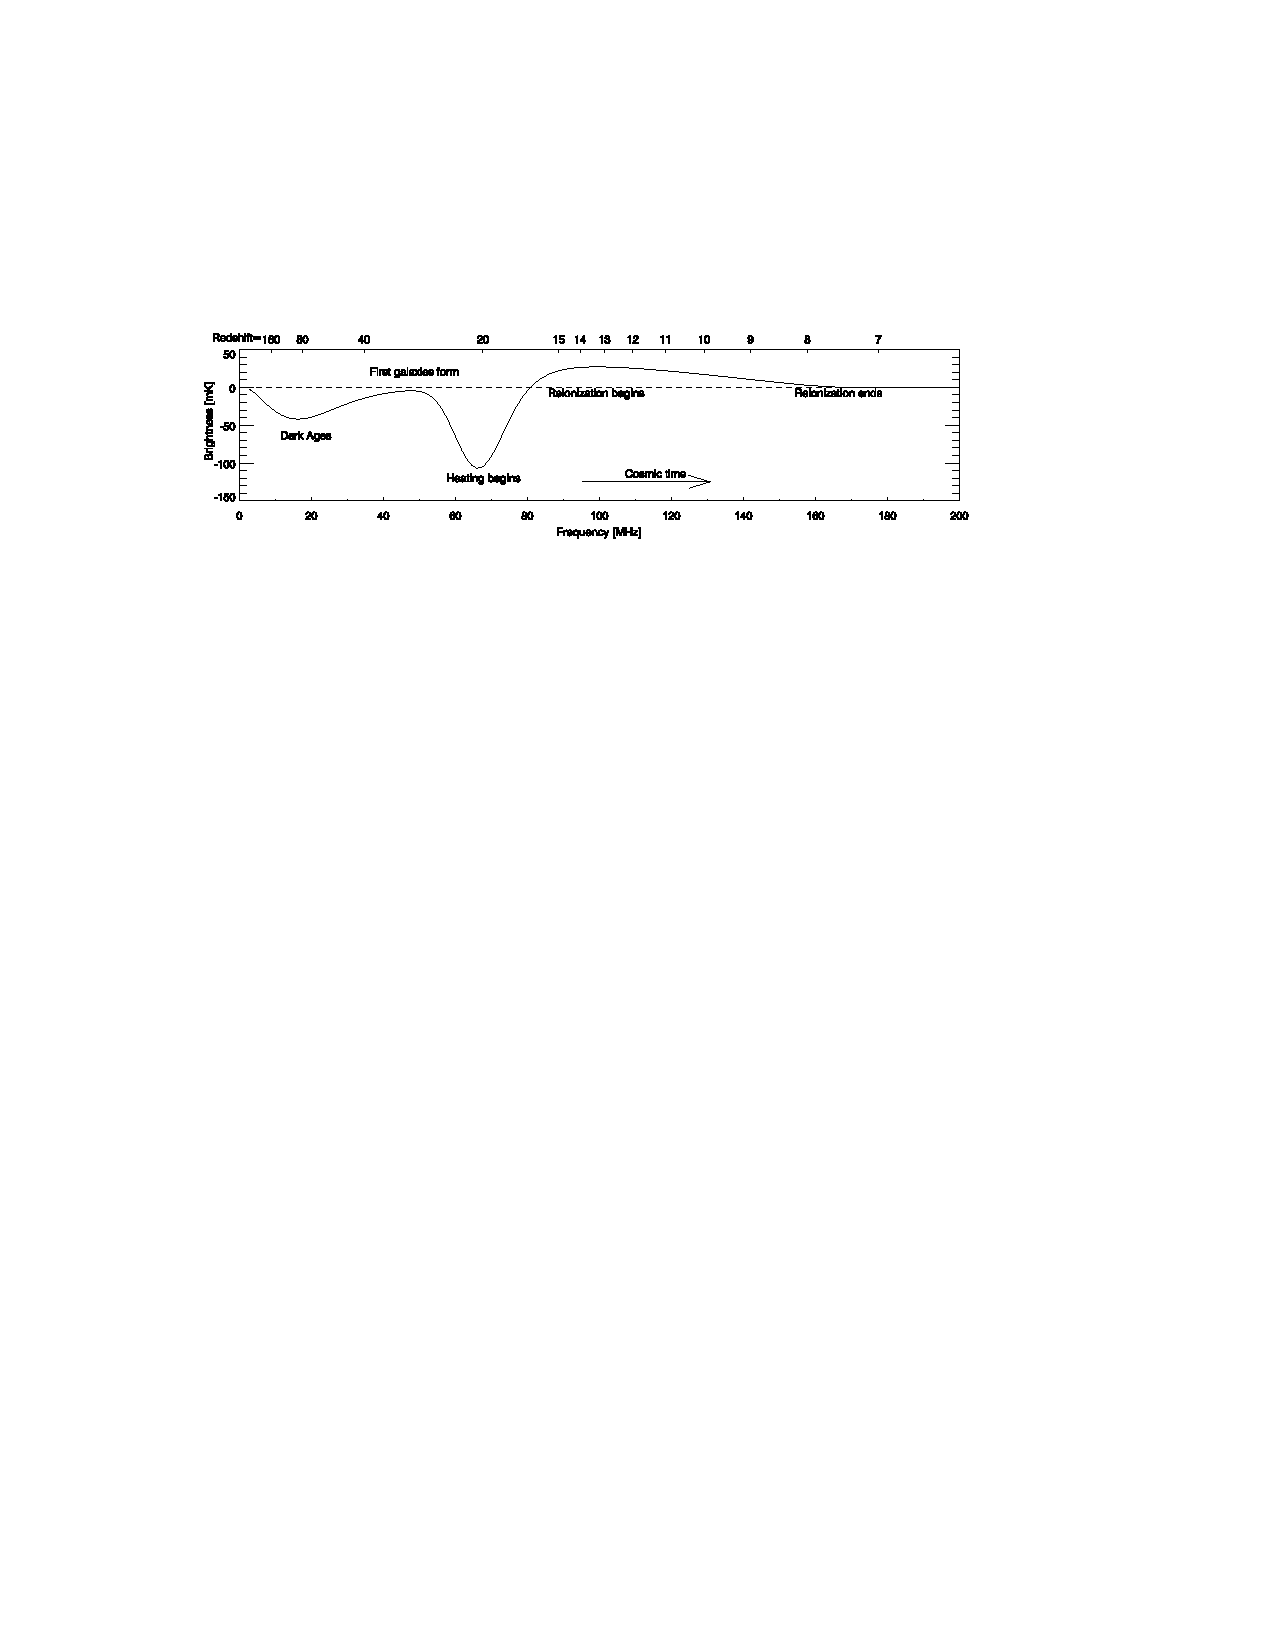
\includegraphics[trim = 0.2cm 0.6cm 0.2cm 0.2cm, scale = 1.0]{Greig/GlobalSignal}
\end{center}
\caption{A representative example of the all-sky averaged (global) 21-cm brightness temperature signal, demarcating the major cosmological transitions. Taken from \cite{Pritchard:2012}.}
\label{fig:global}
\end{figure}

The global signal has been studied extensively in the literature. {\color{red} Use this hook here to add in citations to works investigating the global signal}.

Roughly speaking the global 21-cm signal can be broken up into five major turning points (e.g. \cite{Furlanetto:2006,Pritchard:2010}) corresponding to: (i) a minimum during the dark ages where collisional coupling becomes ineffective, (ii) a maximum at the transition from the dark ages to the Ly$\alpha$ pumping regime (Ly$\alpha$ pumping from the first sources becomes efficient), (iii) a minimum at the commencement of X-ray heating taking the signal back towards emission, (iv) a maximum once the 21-cm signal becomes saturated during the EoR and finally (v) when reionisation is complete. Importantly, both the amplitude of the 21-cm signal as well as the frequency (redshift) of these transitions is strongly dependent on the underlying astrophysical processes. Thus, measuring both the amplitude and frequency of the turning points can reveal information into the underlying astrophysics.

In \cite{Mirocha:2013}, these authors connect these transitions more closely to the astrophysics. The second turning point (end of the dark ages) can, under certain simple assumptions, be used to place limits on the spin temperature, $T_{\rm S}$. Details on $T_{\rm S}$, through equation ({\color{red} should be in an earlier chapter}) can provide an estimate on the angle-averaged intensity of Ly$\alpha$ photons, $J_{\alpha}$. This provides insight into both the number density of sources and their corresponding emission spectrum (e.g. PopIII stars). The relative depth of the third turning point (heating epoch) can be used to place limits on the co-moving heating rate density, that is, the amount of heating that the IGM has undergone owing to heating sources (e.g. X-rays from HMXBs, the ISM or other more exotic scenarios {\color{red} should be discussed in an earlier chapter}). Again, distinguishing the number density and type of sources responsible. Finally, the saturation of the spin temperature, $T_{\rm S}$, during the epoch of reionisation collapses the brightness temperature into an approximate proportionality ({\color{red} cite appropriate equation}, $T_{\rm S} \propto x_{\rm H{\scriptstyle I}}(1+\delta_{\rm nl})$) with the underlying ionisation fraction, $x_{\rm H{\scriptstyle I}}$. Tracking the evolution of the ionised fraction, i.e. the reionisation history, reveals the time-span of reionisation. This reveals insights into the number density of ionising photons produced, and thus the types of sources responsible for reionising the Universe.

Up until very recently, the first transition was typically ignored, as it was assumed that this transition was well understood theoretically. That is, that the dark matter and baryons decoupled from the CMB temperature at the same time, both cooling adiabatically. It turns out that the dark matter decouples earlier than the baryons, meaning the dark matter is colder than the baryons. As such, the baryons can be cooled by a coupling between the dark matter and baryons (e.g. \cite{Tashiro:2014}) altering the amplitude of the 21-cm signal. In addition to this, relative velocity differences between the two fluids (dark matter and baryons) will affect the structure formation on small-scales (e.g. \cite{Tseliakhovich:2010}) again impacting on the temperature of the baryons. These will result in observable differences in the location and amplitude of this first turning point in the global signal, enabling dark matter models to be distinguishable (e.g. \cite{Munoz:2015,Fialkov:2018}).

To highlight the expected variation in the global 21-cm signal as a result of the underlying astrophysical processes, in Figure~\ref{fig:global_vary} we show $\sim~200$ theoretical models of the global 21-cm signal from \cite{Cohen:2017}. Here, the authors explore the maximal variation in the global 21-cm signal when varying the ionisation and heating properties of the astrophysical sources. Some common features in the signal are, the depth of the absorption trough deepens for lower X-ray luminosities (including some models which never appear in emission as a result of inefficient heating) or the turning points push to later times when the minimum masses of sources increases (i.e. require more massive haloes in which stars can form and produce ionising photons).

\begin{figure}[]
\begin{center}
%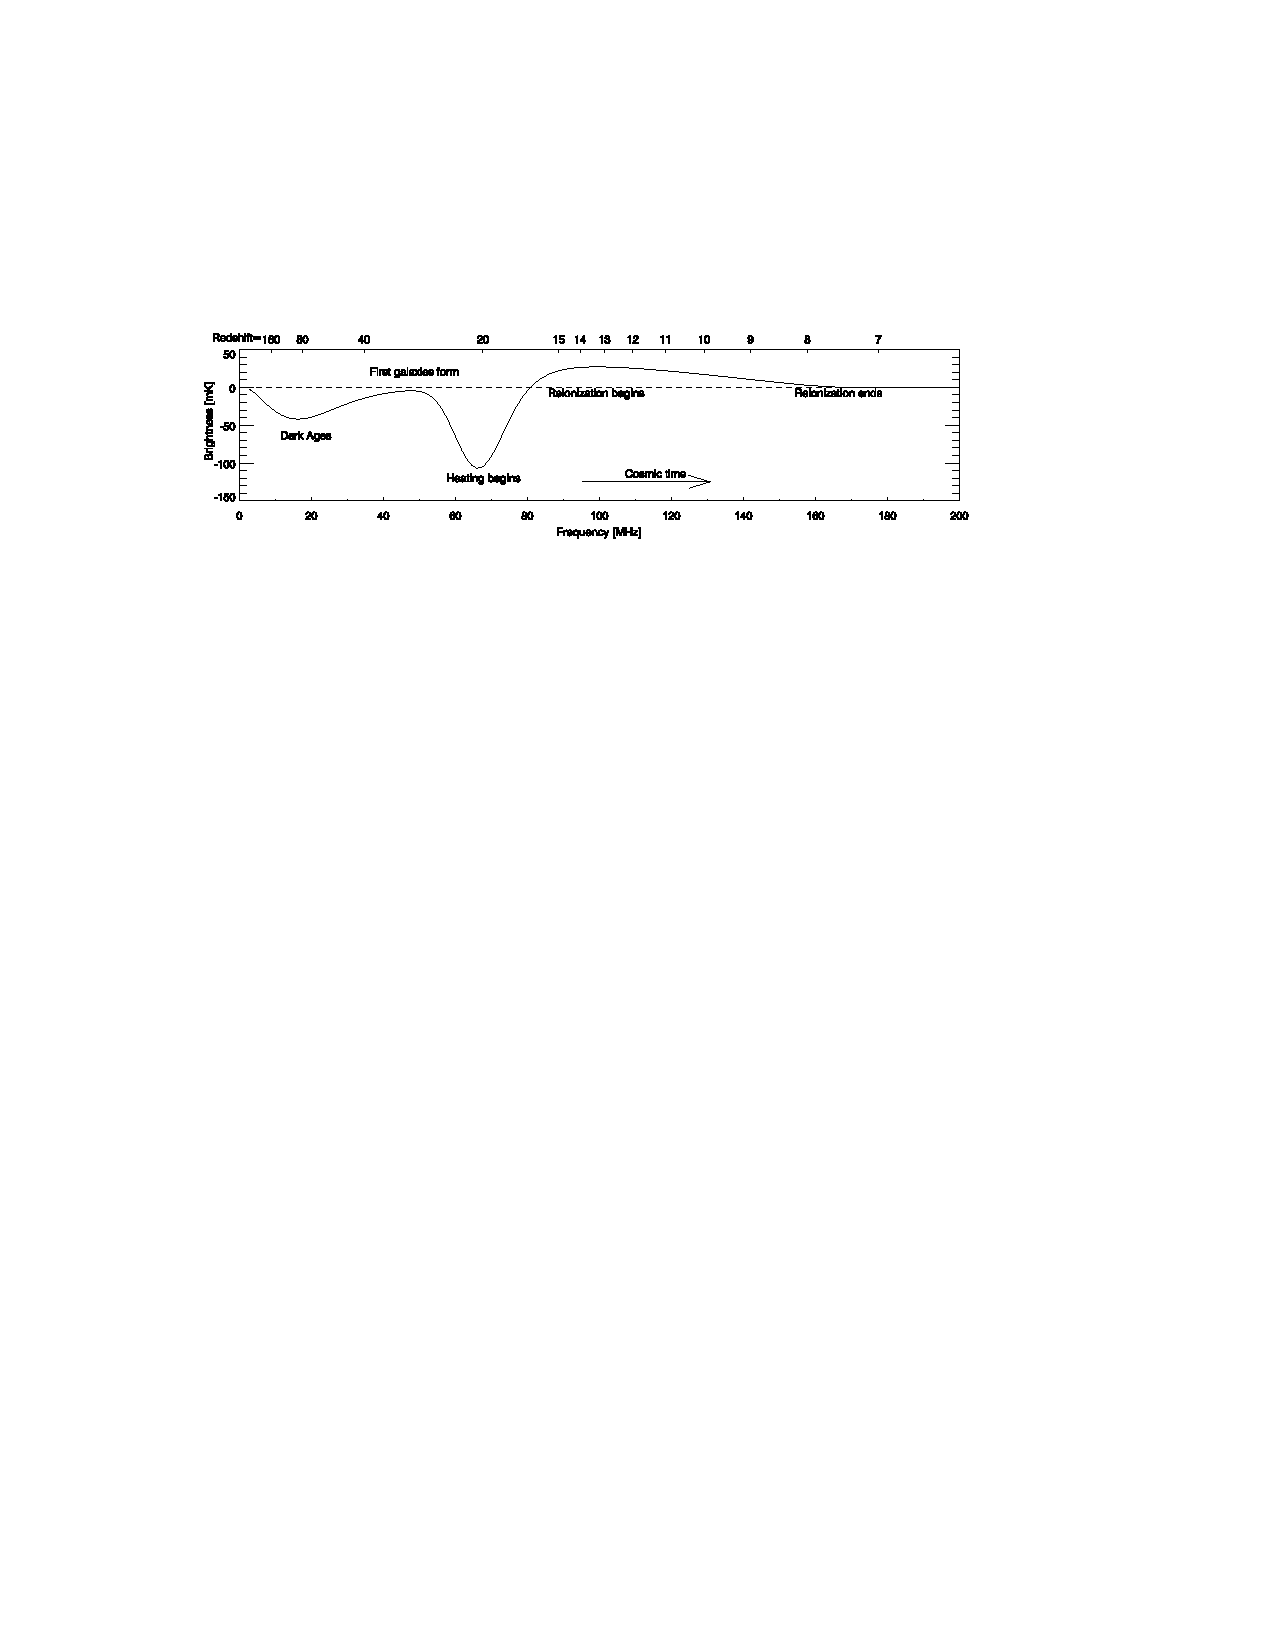
\includegraphics[width=1.\textwidth]{Greig/GlobalSignal}
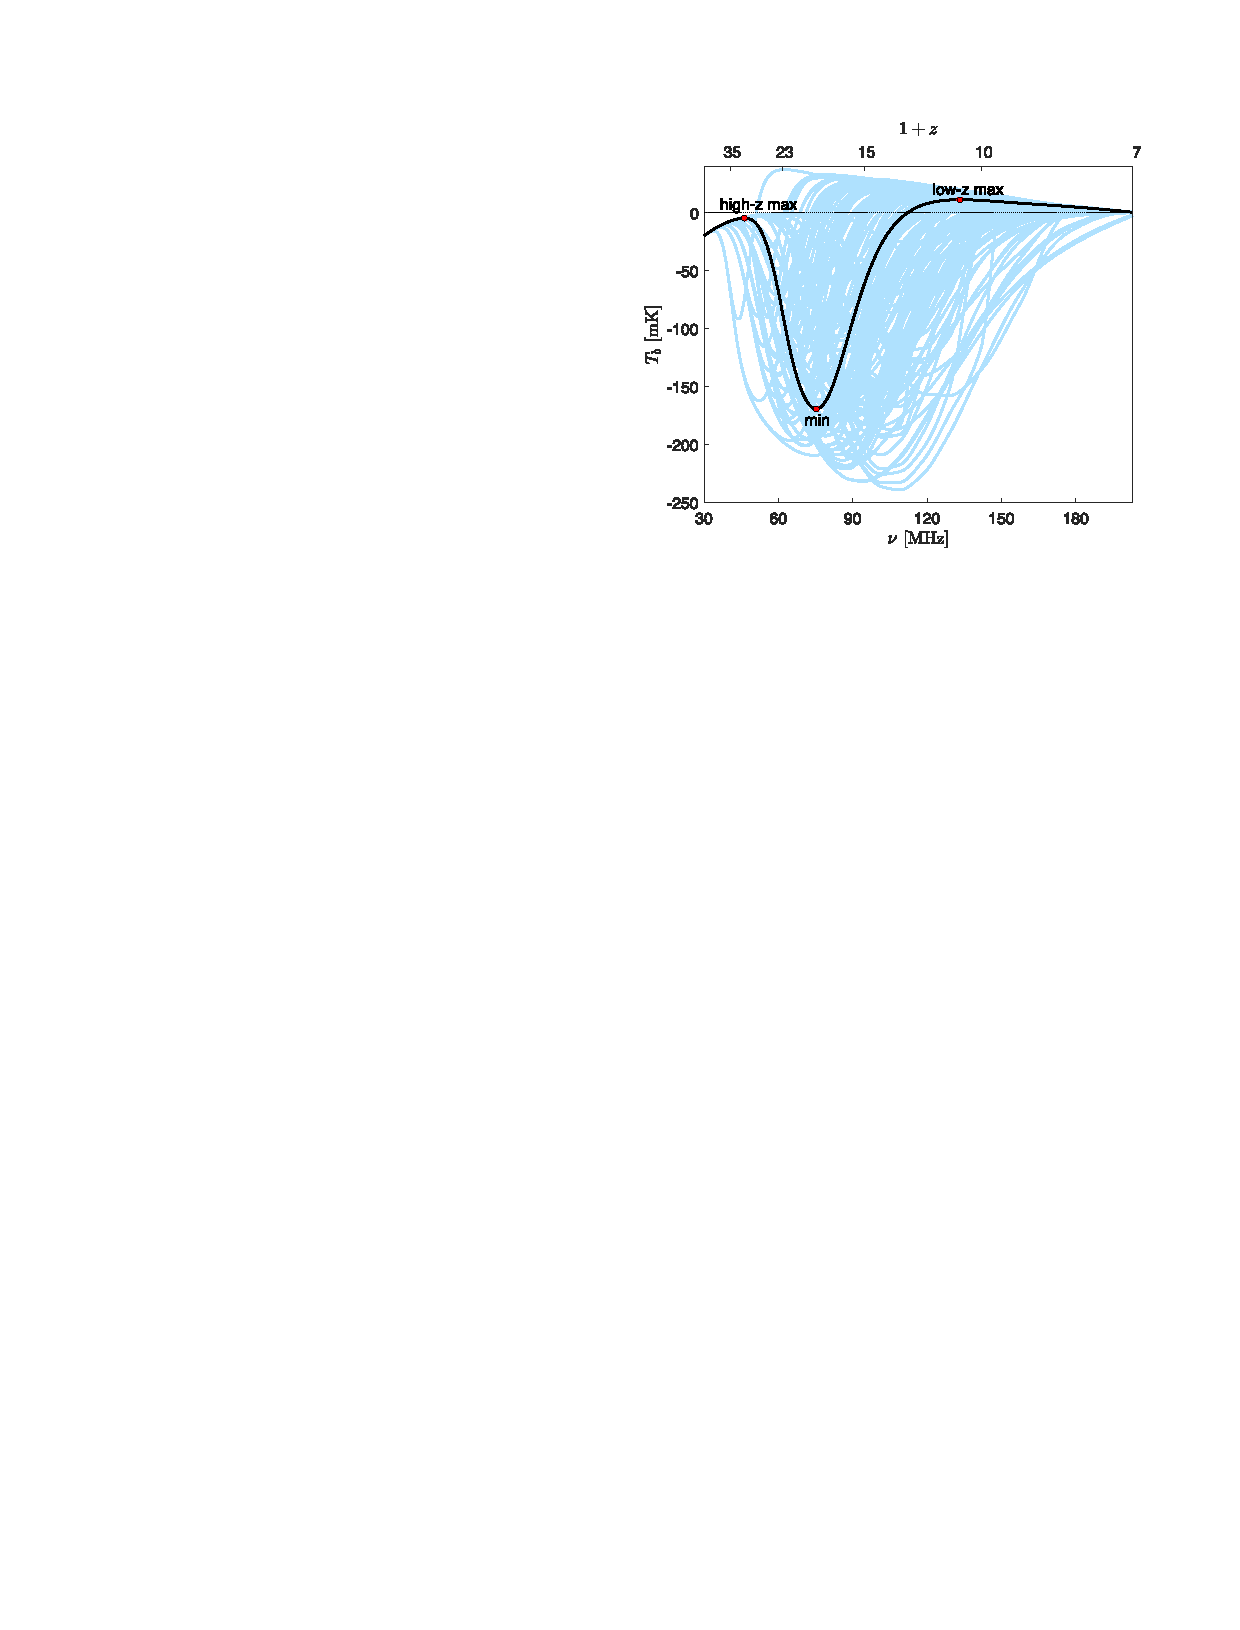
\includegraphics[trim = 0.2cm 0.6cm 0.2cm 0.2cm, scale = 0.9]{Greig/GSVariation}
\end{center}
\caption{The all-sky averaged (global) 21-cm brightness temperature signal obtained when varying the astrophysical parameters in $\sim~200$ theoretical models from \cite{Cohen:2017}.
}
\label{fig:global_vary}
\end{figure}

\subsection{Power spectrum}

After the global signal, the next simplest and most straightforward approach to characterise the 21-cm signal is through the power spectrum. This is the Fourier transform of the 2-point correlation function. Basically, a measure of the excess signal (above random) on all possible spatial scales. The workhorse statistic for any signal containing structural information, the power spectrum is simply the number of modes (in Fourier space) as a function of physical scale (or size). It produces a distribution of modes characterising the amount of structural information which is contained within the signal. The power spectrum is the natural method for observing the 21-cm signal from a radio interferometer, since these measure differences in the arrival times of the cosmological signal between radio dipoles or dishes of some fixed separation. Thus, a radio interferometer is sensitive to the spatial fluctuations rather than the total amplitude.

To obtain the 21-cm power spectrum, we normalise the 21-cm brightness temperature, $\delta T_{b}(\mathbf{x})$ to be a zero-mean quantity, $\delta_{21}(\mathbf{x}) = (\delta T_{b}(\mathbf{x}) - \delta\bar{T_{b}})/\delta\bar{T_{b}}$, which amplifies the fluctuations (spatial information) in the signal. The power spectrum, $P(\mathbf{k})$ is computed by the angle-averaged sum of the Fourier transform of the 21-cm brightness temperature fluctuations via,
\begin{eqnarray}
\langle \delta_{21}(\mathbf{k}_{1})\delta_{21}(\mathbf{k}_{2}) \rangle = (2\pi)^{3}\delta_{D}( \mathbf{k}_{1} + \mathbf{k}_{2})P(\mathbf{k}_{1}),
\end{eqnarray}
where $\delta_{D}$ is the Dirac delta function. Typically, the 21-cm power spectrum is converted into a dimensionless quantity through $\Delta^{2}(\mathbf{k}) = (k^{3}/2\pi^{2})P(\mathbf{k})$. Typically, the Fourier modes are then averaged in spherical shells to obtain the spherically averaged power spectrum, $P(k)$, which considerably improves the overall signal-to-noise, at the cost of averaging over some spatial information. Alternatively, one can also measure the two-dimensional cylindrically averaged power spectrum, $P(k_\parallel,~k_\perp)$ decomposing it into modes perpendicular to the line-of-sight ($k_\perp$; spatially averaging the two dimensional angular modes on the sky in annuli) and along the line-of-sight ($k_\parallel$; in frequency) direction. The strength of the two dimensional 21-cm power spectrum is that most of the contamination of the signal by the astrophysical foregrounds can be contained in what is referred to as the EoR `wedge' while the remaining Fourier modes can be clean tracers of the cosmological signal ({\color{red} cite references and/or subsequent chapter}).

The advantage of the power spectrum over the global signal, is that it provides a measure of the spatial fluctuations in the 21-cm signal. However, it does not encode all the available spatial information from the 21-cm signal. The power spectrum is a measure of how Gaussian the fluctuations are. If these fluctuations were truly Gaussian, the power spectrum would contain all the information, and any higher order $n$-point correlation functions would contain no additional information. The structural complexity of the large and small scale processes of reionisation and the cosmic dawn results in the signal being highly non-Gaussian. As such, the power spectrum does not reveal all available information, meaning there is further constraining power from the higher order $n$-point statistics. In section~\ref{sec:bispectrum} we will return to this. Nevertheless, the power spectrum still contains a wealth of information, and observationally is considerably easier to measure.

\begin{figure}[]
\begin{center}
%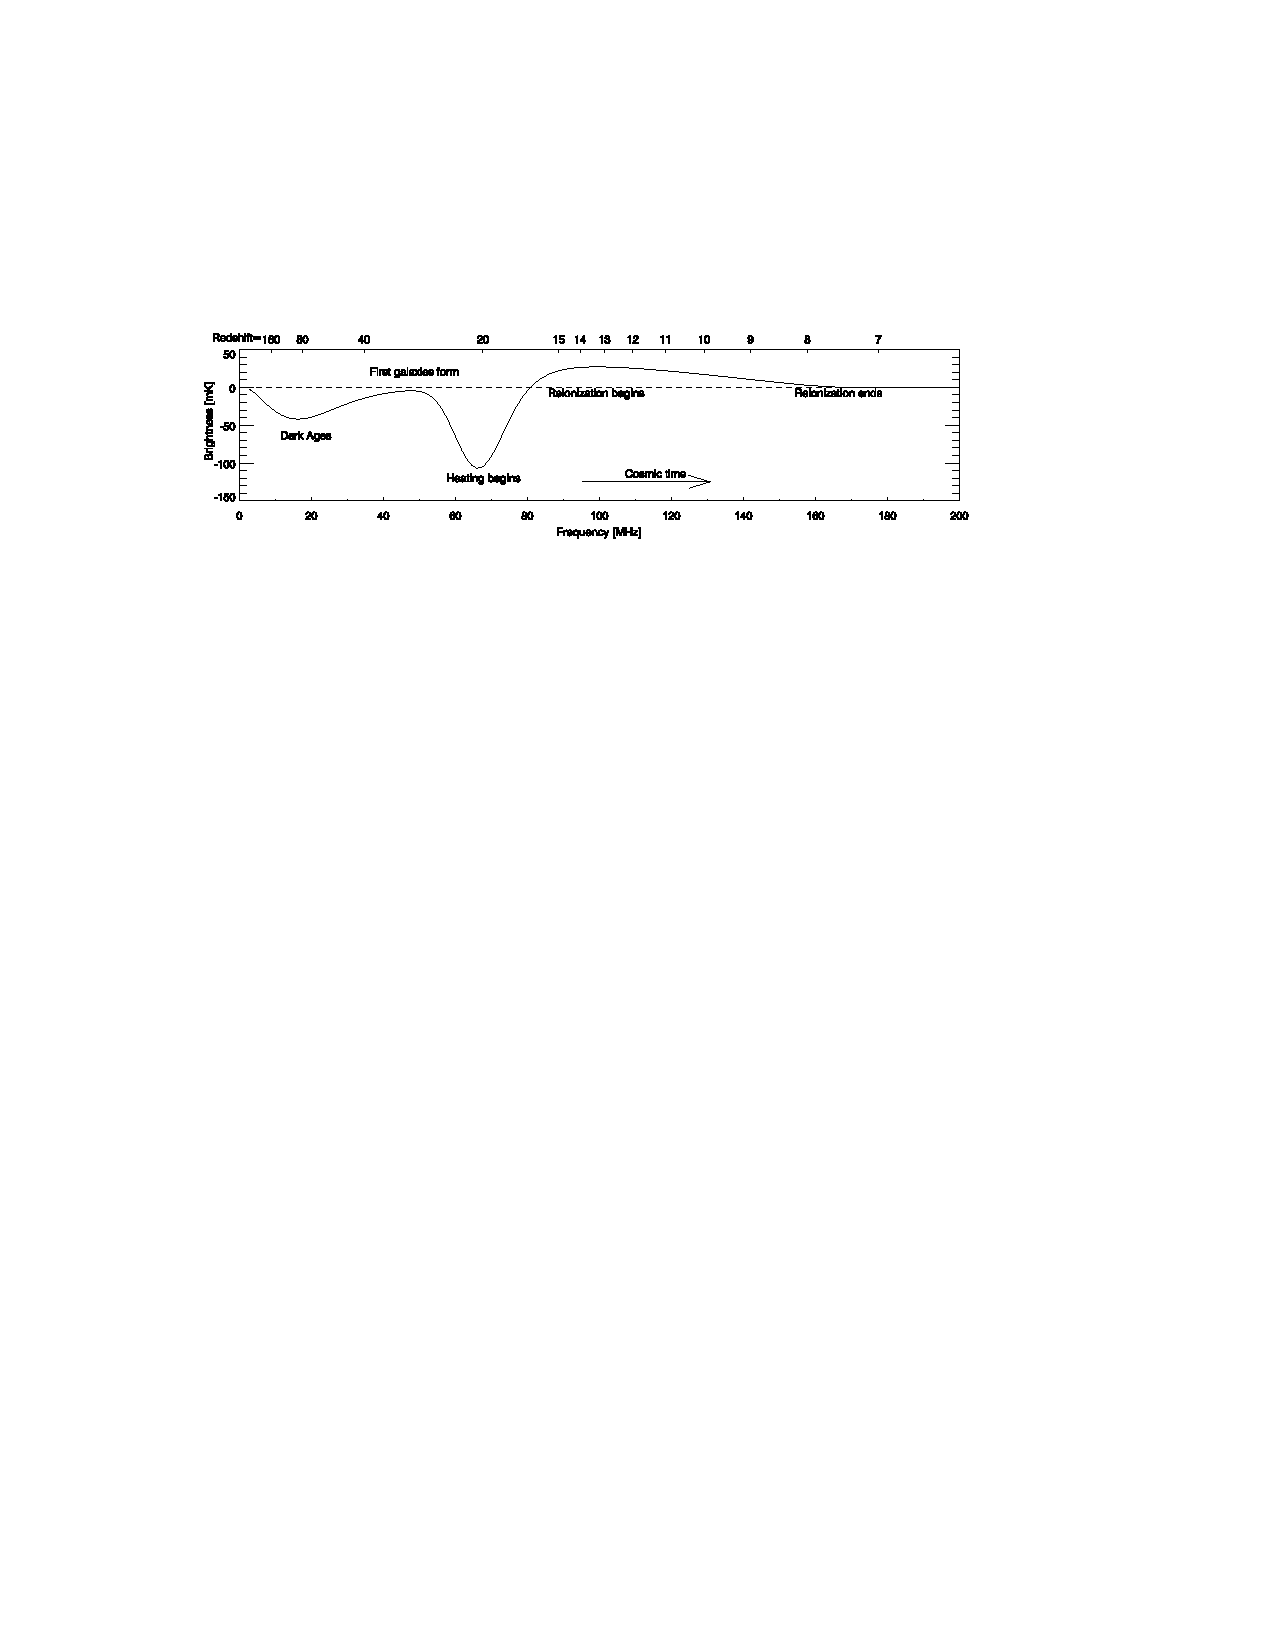
\includegraphics[width=1.\textwidth]{Greig/GlobalSignal}
\includegraphics[trim = 0.2cm 0.6cm 0.2cm 0.2cm, scale = 0.4]{Greig/PSMilestones}
\end{center}
\caption{The 21-cm power spectrum amplitude for two different Fourier modes, $k=0.1$~Mpc$^{-1}$ (solid) and $k=0.5$~Mpc$^{-1}$ (dashed). Peaks in the 21-cm power spectrum amplitude correspond to the different cosmic milestones. Taken from \cite{Mesinger:2016}.}
\label{fig:PSMilestones}
\end{figure}

The sensitivity of the 21-cm power spectrum to the underlying astrophysics can be highlighted when we decompose the 21-cm brightness temperature fluctuations through a perturbative analysis. In doing so, we can recover the following (see e.g. {\color{red} needs references}),
\begin{eqnarray}
\delta_{21} \propto C_{b}\delta_{b} + C_{x}\delta_{x} + C_{\alpha}\delta_{\alpha} + C_{T}\delta_{T} - \delta_{\partial v},
\end{eqnarray}
Simply put, fluctuations in the 21-cm brightness temperature field, $\delta_{21}$, are driven by a sum of contributions from the underlying density field, $\delta_{b}$, the ionisation fraction $\delta_{x}$, the Ly$\alpha$ coupling co-efficient, $\delta_{\alpha}$, the temperature of the neutral hydrogen $\delta_{T}$ and line-of-sight peculiar velocity gradient, $\delta_{\partial v}$. Computing the power spectrum then measures the combined signal from the power spectra of each field as well as the cross-power spectra of each. Thus, if we measure the 21-cm power spectrum across cosmic time, we will be sensitive to both the epochs when each component dominates (similar to the global signal) and also the spatial scales on which the signal is strongest. This, similar to the global signal is depicted in Figure~\ref{fig:PSMilestones}.

However, rather than using one single Fourier mode, we have a range of spatial scales over which to recover astrophysical information. This provides access to both the small-scale and large-scale physical processes. For example, during the EoR, the 21-cm power spectrum is dominated by the contribution from the ionisation field, which contains particular structural information on the reionisation process due to the characteristic size of the H$_{\rm \scriptsize II}$ regions as well as their clustering ({\color{red} cite references}). Similar is true for both the heating or Ly$\alpha$ coupling epochs, whereby the structural information provides insights into the intensity of the radiation, and the number density of sources producing it.

\begin{figure}[]
\begin{center}
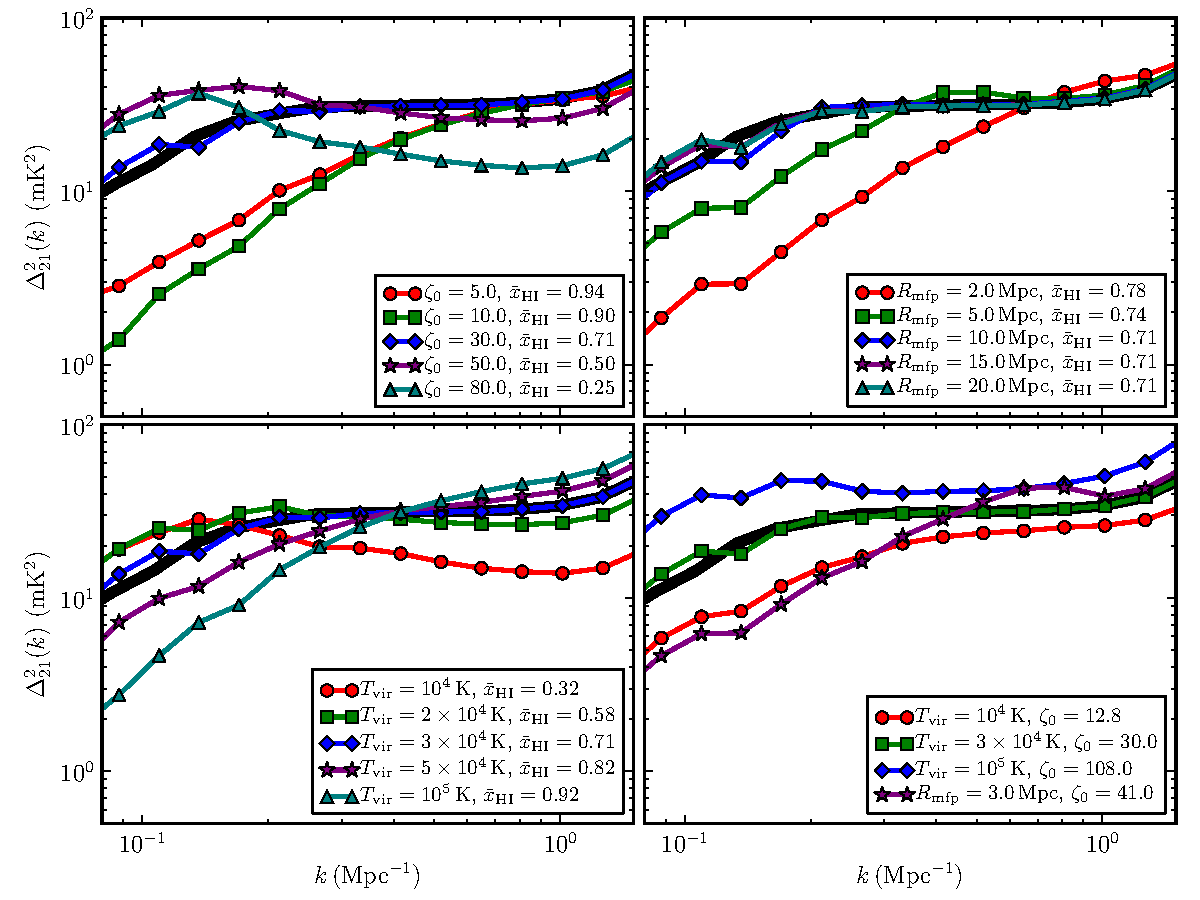
\includegraphics[trim = 0.2cm 1cm 0.2cm 0.2cm, scale = 0.75]{Greig/ParameterVariation_z9_0_book}
\end{center}
\caption{The three dimensional spherically averaged 21-cm power spectrum at $z=9.0$ when varying astrophysical parameters controlling different astrophysical processes, assuming $T_{\rm S} \gg T_{CMB}$~(\cite{Greig:2015}). Top left: the number of ionising photons produced per baryon (ionising efficiency, $\zeta$), top right: maximum ionising photon horizon (proxy for maximum allowable bubble size, $R_{\rm mfp}$) and bottom left: minimum mass of halo hosting star-forming galaxy (represented here as $T_{\rm vir}$). Bottom right: several models at the same ionisation fraction.}
\label{fig:PSvariation}
\end{figure}

In Figure~\ref{fig:PSvariation} we show the variation in the three dimensional spherically averaged 21-cm power spectrum at a single redshift ($z=9$) when varying three different astrophysical parameters under the assumption of $T_{\rm S} \gg T_{CMB}$(see e.g. \cite{Greig:2015}). Inset tables correspond to the parameter being varied and the resultant IGM neutral fraction (stage of reionisation). In the top left panel, we vary the ionising efficiency, $\zeta$, a proxy for the number of ionising photons produces by the sources. The shape of the 21-cm power spectrum differs considerably with ionising efficiency. In the early stages, the 21-cm PS matches the density (matter) power spectrum, while in the latter stages its follows the ionisation field {\color{red} this surely has been discussed in detail already and I don't have to elaborate on it?}. 

Similar behaviour is observed for varying $T_{\rm vir}$, a proxy for the minimum mass of halos hosting star-forming galaxies. Increasing this threshold, results in fewer sources to contribute to reionisation. In the top right panel, the maximum photon horizon, $R_{\rm mfp}$, is varied. Essentially, in this specific work it acts as a maximum allowable bubble size. Note that in this case, the change in $R_{\rm mfp}$ does not alter the neutral fraction strongly, thus the changes in the 21-cm power spectrum are purely as a result in changes to the size of the ionised regions. Finally, in the bottom right we highlight astrophysical models with the same IGM neutral fraction (i.e. the same stage of reionisation). Despite being at the same point in reionisation, the amplitude and shape of the 21-cm power spectrum differs considerably, highlighting the sensitivity of the 21-cm power spectrum to the underlying astrophysical parameters. 

While this example is only for the epoch of reionisation, the same strong sensitivity of the 21-cm power spectrum to the underlying astrophysics is true for both the heating or Ly$\alpha$ coupling epochs (see e.g. {\color{red} citations}). This highlights the strength and utility of the 21-cm power spectrum for recovering the astrophysical information. As such numerous authors have explored the impact of various astrophysical processes on the 21-cm power spectrum. {\color{red} refer to a variety of papers here, and potentially highlight the specific process used}.

\subsection{Bispectrum} \label{sec:bispectrum}

The logical extension beyond the power spectrum, the bispectrum, $B$, is simply the Fourier transform of the 3-point correlation function,
\begin{eqnarray}
\langle \delta_{21}(\mathbf{k}_{1})\delta_{21}(\mathbf{k}_{2})\delta_{21}(\mathbf{k}_{3}) \rangle = (2\pi)^{3}\delta_{D}( \mathbf{k}_{1} + \mathbf{k}_{2} + \mathbf{k}_{3})B(\mathbf{k}_{1},\mathbf{k}_{2},\mathbf{k}_{3}),
\end{eqnarray}
where the $\delta_{D}$ enforces that the Fourier modes must form closed triangles. It measures the excess probability of the underlying quantity as a function of three spatial positions in real space. The bispectrum provides a scale-dependent measure of the non-Gaussianity of the 21-cm signal, and as such contains additional astrophysical information beyond that held in the power spectrum. However, it suffers from lower signal-to-noise as there are less modes to average over to boost the signal.

Whereas the power spectrum is relatively trivial to interpret as it is a measure of the power over a single length scale, $k$, the bispectrum is the measure of power over all possible triangle configurations that satisfy the closure condition from $\delta_{D}$. Thus in order to simplify the interpretation of the bispectrum, it is common to consider several simplified triangle configurations. These are typically: (i) the equilateral triangle ($k_{1}  = k_{2} = k_{3}$), (ii) the isosceles triangle ($k_{1} > k_{2} = k_{3}$), (iii) folded triangle ($k_{1} = 2k_{2} = 2k_{3}$), (iv) elongated triangle ($k_{1} = k_{2} + k_{3}$) and (v) the squeezed triangle ($k_{1} \simeq k_{2} \gg k_{3}$). Each, corresponds to different physical properties of the real-space field.

While a detailed discussion of the 21-cm bispectrum is beyond the scope of this chapter, it is fruitful to provide a brief explanation and example of the various configurations (see for example \cite{Lewis:2011} and \cite{Watkinson:2019} for more detailed discussions). The equilateral configuration is essentially an extension of the power spectrum, in the sense that it is expressed as a single amplitude scale, $k$. Generally speaking, it produces the largest amplitude signal and as such is the most commonly studied configuration. It is sensitive to the spherical symmetry of the 21-cm signal such as the scale of the ionised H$_{\rm \scriptstyle II}$ regions during reionisation or the hot/cold spots due to IGM heating. Typically its amplitude grows during the EoR as the signal becomes more non-Gaussian due to the topology of the ionisation field. Shifting towards isosceles or folded triangles, these become more sensitive to planar or filamentary structures in the underlying 21-cm signal. Thus as the topology of either the ionised or X-ray heated regions deviate away from spherical symmetry (i.e. either multiple contributing sources or overlap of ionised regions) the signal should increase with increasing angle. The squeezed limit correlates the small-scale signal from two modes with a large-scale mode, for example capturing the impact of the large-scale environment (i.e. from X-ray heating) on the small-scale power spectrum (i.e. source clustering).

In addition to the structural information in the bispectrum amplitude, the relative sign of the bispectrum equally reveals insight into the underlying processes. As discussed in \cite{Majumdar:2018}, the sign of the bispectrum during reionisation can distinguish between whether the non-Gaussianity is driven by the topology of the ionised regions (where the bispectrum is negative) compared to being driven by the matter and cross-bispectra (where it is positive).

In Figure~\ref{fig:EqBS}, we compare the equilateral bispectrum at $z=7$, 8 and 9 from \cite{Shimabukuro:2017} for differing ionising efficiency, $\zeta$. For decreasing $\zeta$, the amplitude of the bispectrum increases due to its amplitude being dependent on the ionisation fraction. Thus, different reionisation models are easily distinguishable by the 21-cm bispectrum.

\begin{figure}[]
\begin{center}
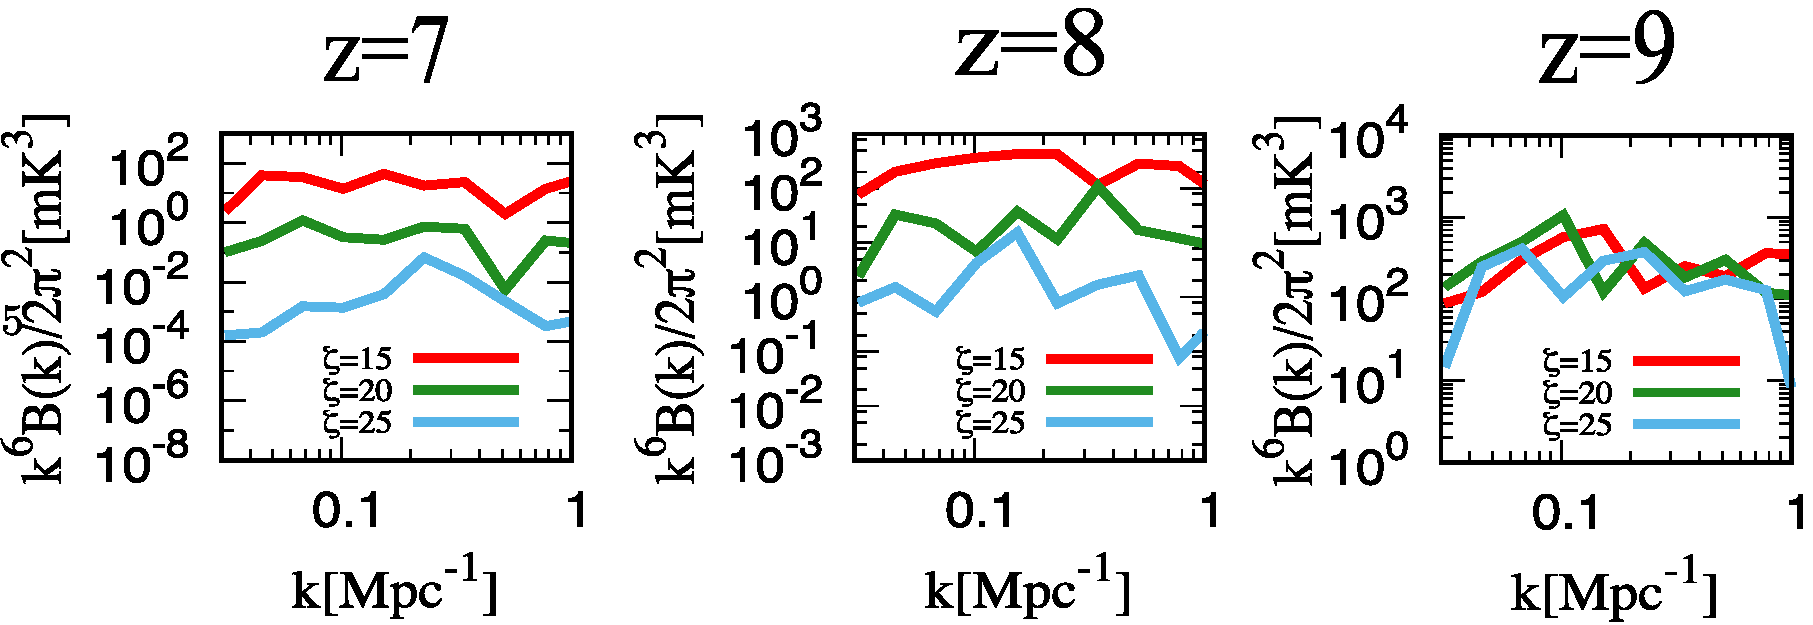
\includegraphics[trim = 0.2cm 1cm 0.2cm 0.2cm, scale = 0.5]{Greig/EqBS}
\end{center}
\caption{Variation in the amplitude of the equilateral bispectrum at $z=7$, 8 and 9 for different ionising efficiencies, $\zeta$, from \cite{Shimabukuro:2017}.}
\label{fig:EqBS}
\end{figure}

Note that the bispectrum is not measured independently from the power spectrum, thus both the power spectrum and bispectrum can be combined to considerably improve our understanding of the underlying astrophysics ({\color{red} can refer to the equivalent case for cosmology where the combination of the two improve the constraining power}).

In recent times, the 21-cm bispectrum has gained considerable traction in interpreting the astrophysics of reionisation and the cosmic dawn. {\color{red} add in citations here works exploring the bispectrum, and quickly what they are exploring}.

Some examples of the exploration of the 21-cm bispectrum. \cite{Watkinson:2019,Watkinson:2017,Shimabukuro:2016}

\subsection{Trispectrum} \label{sec:bispectrum}

I am certain someone looked at the trispectrum...

\subsection{One-point statistics}

Rather that measuring the Fourier transform (e.g. power spectrum) of the 21-cm brightness temperature signal, $\delta_{21}(\mathbf{x})$, we can instead measure the one-point statistics (or moments) of the probability distribution function (PDF). In fact, we have already discussed the lowest order one-point statistic, that is, the mean of $\delta T_{b}(\mathbf{x})$ given by the global signal (see \ref{sec:global}).  These one-point statistics of the PDF essentially measure the deviations away from a fully Gaussian PDF, thus they are by definition sensitive to the non-Gaussian nature of the 21-cm signal. Generally speaking, the one-point statistics of $\delta T_{b}(\mathbf{x})$ are given by,
\begin{eqnarray}
m_{n} = \frac{1}{N}\sum^{N}_{i=0}(\delta T_{b}(\mathbf{x_{i}}) - \bar{\delta T_{b}})^{n},
\end{eqnarray}
where $m_{n}$ is the $n$-th order moment and $N$ is the number of pixels over which the signal is measured. For the 21-cm signal, these moments would be generated from the observed two-dimensional tomographic maps of the 21-cm signal.

The next lowest order statistic of the PDF following the mean is the variance, $\sigma^{2}$. The variance is equivalent to the average of the power spectrum over all Fourier modes, $k$,
\begin{eqnarray}
\sigma^{2} = (\bar{\delta T_{b}})^{2} \int \frac{d^{3}k}{(2\pi)^{3}} P(\mathbf{k}).
\end{eqnarray}
As it is the average over all spatial information, the variance itself is less sensitive to the underlying astrophysics than the power spectrum. However, the strength of one-point statistics shines through when using the higher order moments in combination with the variance (or power spectrum). The next two higher order moments are referred to as the skewness and the kurtosis. Equivalent to the variance's relation to the power spectrum, the skewness and kurtosis are the average over all Fourier modes of the bispectrum and trispectrum respectively (the three and four-point correlation functions). As such, whereas the power spectrum only measures the 2-point correlations, the skewness and kurtosis reveals insights from the non-Gaussian properties of the 21-cm signal.

\begin{figure}[]
\begin{center}
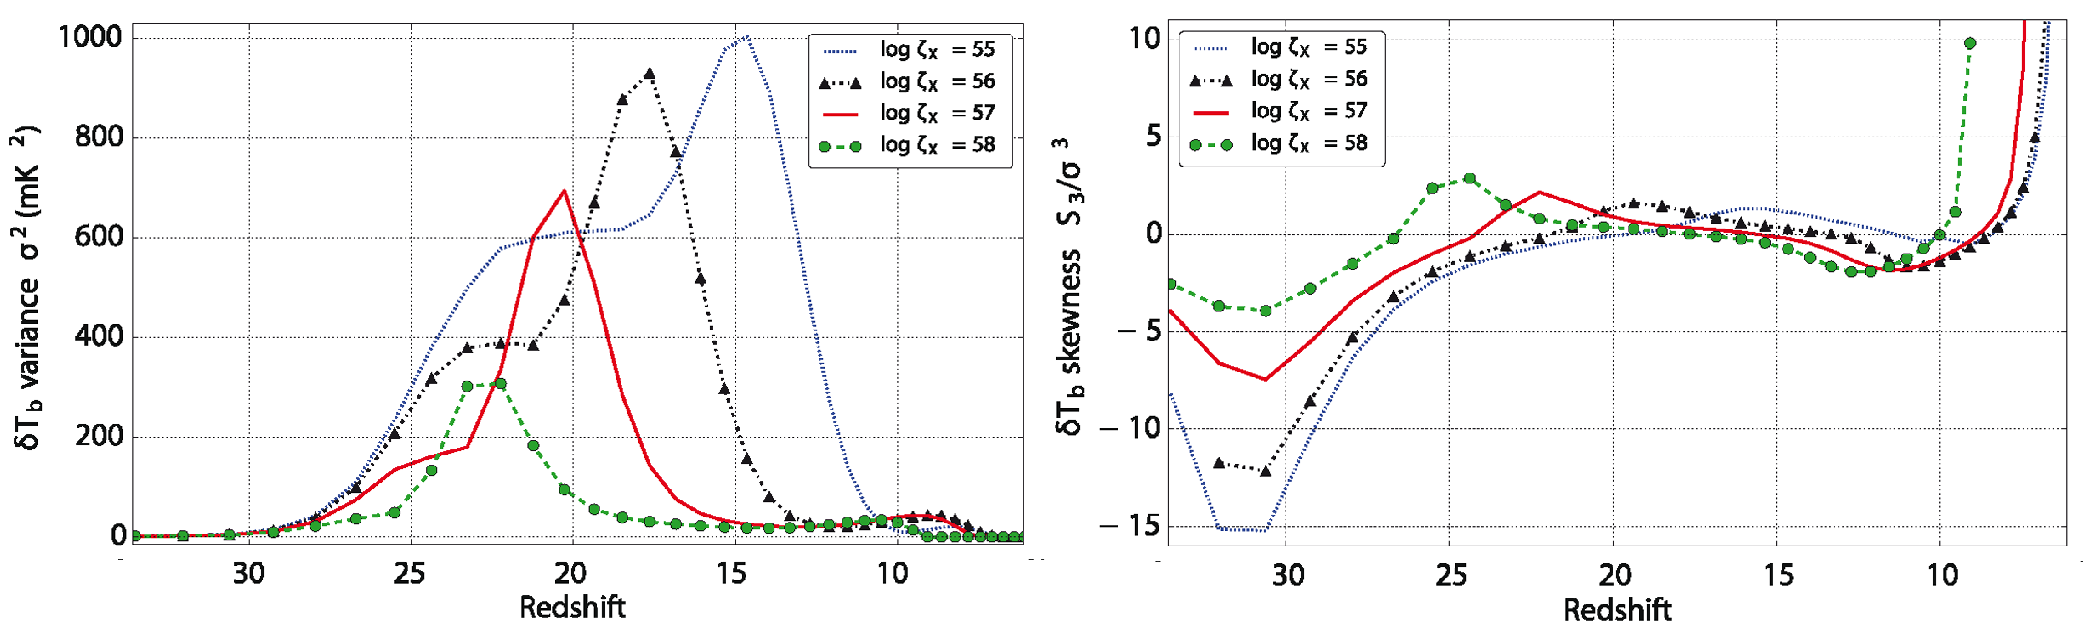
\includegraphics[trim = 0.2cm 1cm 0.2cm 0.2cm, scale = 0.45]{Greig/Skewness}
\end{center}
\caption{The variance (left) and normalised skewness (right) of the 21-cm brightness temperature when varying the efficiency of X-ray heating in the IGM from \cite{Watkinson:2015}.}
\label{fig:skewness}
\end{figure}

The amplitude of the variance is sensitive to differences in the 21-cm brightness temperature. For example, during the EoR, as the number of ionised regions increases (i.e. the contrast between the 21-cm signal from the neutral regions compared to zero signal from the ionised regions) the variance increases. It subsequently turns over as most of the volume is ionised. The skewness is a measure of the asymmetry of the underlying PDF. A negative skewness corresponds to a longer tail towards a lower amplitude signal and a positive skewness corresponds to a longer tail towards higher amplitude signals. The kurtosis is essentially a measure of the outliers of the distribution, with increasing positive (negative) kurtosis corresponding to larger positive (negative) amplitude outliers.

Figure~\ref{fig:skewness} shows an example of both the variance (left) and normalised skewness (right panel) of the 21-cm brightness temperature under different levels of X-ray heating. For increasing X-ray efficiencies (i.e. increase heating) the peak of the variance decreases in amplitude while shifting to earlier times. Increasing the efficiency allows the X-ray heating to occur earlier, reducing the contrast between the $T_{\rm CMB}/T_{\rm S}$ resulting in a lower amplitude peak in the variance. This same behaviour equally results in larger skewness for decreasing X-ray efficiency, owing to a more asymmetric PDF of 21-cm brightness temperatures due to the increasing contrast in $T_{\rm CMB}/T_{\rm S}$. Clearly from Figure~\ref{fig:skewness} it can be seen that these one-point statistics are capable of distinguishing between different astrophysical models.

{\color{red} Some (but not all) references for the one-point statistics. \cite{Harker:2009,Patil:2014,Kittiwisit:2016,Kubota:2016,Watkinson:2014,Shimabukuro:2015,Ross:2017}}

\subsection{Wavelets}

Thus far we have only considered either real-space quantities such as the one-point statistics or the Fourier transform of the $n$-point correlation functions (i.e. the power spectrum and bispectrum). The Fourier transform measures the amplitude of the fluctuations of a given spatial scale, and in order to increase the signal-to-noise we must average the signal over all line-of-sight modes within some observed bandwidth. As a result, we average over modes containing different redshift evolutions and thus increase the bias of the signal. This can be minimised somewhat, for the case of the power spectrum, by averaging the signal over relatively narrow observing bandwidths. However, it still results in some loss in fidelity of the signal.

Instead, in \cite{Trott:2016} the authors explore the potential usage of wavelets, which provide multiple alternatives to the Fourier basis set. Specifically, they explored the application of the Morlet Transform. This provides a family of curves which provide the ability to localise the 21-cm signal both spatially and in frequency. In doing so, the equivalent to the power spectrum, the Morlet power spectrum is capable of providing an unbiased estimator which maximises the three dimensional nature of the 21-cm signal. Preliminary analysis shows that the Morlet power spectrum performs more optimally than the Fourier power spectrum. A physical interpretation of the Morlet power spectrum in the context of the evolution of the 21-cm signal has yet to be explored.

\subsection{Topological measurements of the 21-cm signal}

All previous approaches discussed up till this point have characterised the 21-cm signal using some form of statistical analysis, on the basis of maximising the signal-to-noise. However, the most advanced radio interferometers ({\color{red} do I need to name them or refer to future chapter?}) should enable two dimensional images of the 21-cm signal. These images will contain the complicated morphology of the hot/cold patches of the 21-cm brightness temperature throughout the history of reionisation and the cosmic dawn. The relative sizes, shapes and clustering of these hot/cold patches can reveal numerous insights into the underlying astrophysical processes, such as the number density of sources, their contribution to the heating/ionisation of the IGM and the shape of the emitted spectrum of radiation. The study of these geometric shapes in mathematics is referred to as topology.

Topological studies of reionisation and the cosmic dawn are complimentary to the statistical methods described above. For example, reionisation proceeds through three main stages (e.g. \cite{Gnedin:2000,Furlanetto:2016}): pre-overlap, over-lap and post-overlap. In pre-overlap, the first ionised H {\scriptsize II} regions (or bubbles) grow completely in isolation roughly until $x_{\rm HI} \geq 0.1$. Over-lap ($ 0.9 \geq x_{\rm HI} \geq 0.1$) describes the merging of these ionised bubbles into essentially a single large connected ionised region. Finally, post-overlap $x_{\rm HI} \geq 0.9$ corresponds to the breaking down of the last remaining patches of neutral IGM into smaller and smaller islands. Topological studies are capable of breaking down these transitions by describing the ratios of ionised and neutral regions, how the ionised (or neutral) regions are connected together and how they are embedded in the larger structures as they form. This provides unique insights into the reionisation epoch not available from statistical methods.

There are numerous methods to attempt to characterise the topology of the 21-cm signal. Below, we summarise several of the main approaches taken in the literature. Fundamental to topological studies is the definition of how to identify regions of interest. Typically, a threshold value is required, with the quantity above/below this threshold being used to distinguish the two regions.

\subsubsection{Genus or the Euler characteristic}

The genus, $g$, is a topological property that defines the number of cuts one can make to an object (i.e. H {\scriptsize II} region) without dividing it into independent disconnected sub-regions. It can simply be expressed as,
\begin{eqnarray}
g = N_{\rm >th} - N_{\rm < th}
\end{eqnarray}
where $N_{\rm >th}$ and $N_{\rm < th}$ are the number of connected (or fully enclosed) regions above and below the threshold value for identification. By gradually increasing the threshold value from some initial starting value, a genus curve is constructed, which is a measure of the connectedness of the quantity as a function of different threshold values (e.g. $x_{H {\rm \scriptsize I}}$, $\delta T_{b}$). Typically, these threshold values are expressed in units of the standard deviation from the mean.

The genus has been explored, both in two and three dimensions, either in the context of the ionised (or neutral) field (\cite{Gleser:2006,Lee:2008,Friedrich:2011}) or the 21-cm brightness temperature field (\cite{Hong:2014,Wang:2015}). However, it has yet to be explored in the context of the heating epoch (i.e. $T_{\rm S} \gg T_{\rm CMB}$ is typically assumed). For a purely Gaussian field, the genus curve is symmetric around zero. Thus deviations from symmetry highlight the non-Gaussianity of the 21-cm signal. 

Differences in the evolution in the amplitude of the genus as a function of threshold density can distinguish different source biases and ionising efficiencies. For example, reionisation driven by larger, more biased sources exhibits a different topology than one driven by numerous fainter sources. This appears as changes in the amplitude of the genus as a function of threshold. When the ionised regions are isolated, the genus amplitude is higher than when they begin to overlap (as the total number of isolated ionised regions decreases).

\subsubsection{Minkowski functionals}

A more generalised description of the geometry or topology of the 21-cm signal can be obtained from what are referred to as Minkowski functionals. These are well known concepts from the branch of mathematics known as integral geometry. Three dimensional space is completely defined by four Minkowski functionals. Used heavily in cosmology, in particular large-scale structure {\color{red} need to add citations?}, recently they have gained favour for describing the topology of reionisation \cite{Gleser:2006,Friedrich:2011,Yoshiura:2017,Chen:2018}.

For a zero mean scaler function, $u(x)$, (e.g. $\delta T_{\rm b}$) within a volume, $V$, and standard deviation, $u$, we can define an excursion set, $F_{\nu}$, which contains all points that satisfy the threshold, $u(x) \geq \nu\sigma$, where $\nu = u_{\rm th}/\sigma$ and $u_{\rm th}$ is the threshold value. Mathematically, this gives rise to the following Minkowski functionals,
\begin{eqnarray}
V_{0}(\nu) = \frac{1}{V}\int_{V} {\rm d^3}x\,\Theta\left[u(x) - \nu \sigma\right] \\
V_{1}(\nu) = \frac{1}{6V}\int_{\partial F_{\nu}} {\rm d}s \\
V_{2}(\nu) = \frac{1}{6\pi V}\int_{\partial F_{\nu}} {\rm d}s\,\left[\kappa_{1}(x) + \kappa_{2}(x)\right] \\
V_{3}(\nu) = \frac{1}{4\pi V}\int_{\partial F_{\nu}} {\rm d}s\, \kappa_{1}(x)\kappa_{2}(x).
\end{eqnarray}
Here, $\Theta$ is the Heaviside step-function, $\partial F_{\nu}$ is the surface of the excursion set, ${\rm d}s$ is the surface element and $\kappa_{1}(x)$ and  $\kappa_{2}(x)$ are the principle curvatures (inverse of the principle radii) at $x$. The zeroth Minkowski functional, $V_{0}$, corresponds simply to the total volume of the excursion set (i.e. volume above the threshold value), $V_{1}$ and $V_{2}$ correspond to the total surface and mean curvature of the excursion set while $V_{3}$ is the integrated Gaussian curvature over the surface or the Euler characteristic (also $\chi$). The Euler characteristic is related to the genus, $g$, via $V_{3} = 2(1-g)$ thus it effectively describes the shape of the excursion set. Thus, the full set of Minkowski functionals contain additional information beyond that of just the genus.

Generally speaking the following behaviour is expected of the Minkowski functionals throughout reionisation and the cosmic dawn. $V_{0}$ describes the volume contained above/below the threshold value. For example, if $V_{0} \sim 0.5$ at $\delta T_{\rm b} = 0$ this implies the number of hot/cold patches are roughly equal. The $V_{0}$ curve will move from left to right (to increasing $\delta T_{\rm b}$) as heating occurs. $V_{1}$ (reflected in $V_{2}$) exhibits a similar shift to higher $\delta T_{\rm b}$, however it is initially strongly peaked with a high density tail containing the heated regions. This peak smooths out over a broader range of $\delta T_{\rm b}$ as heating continues. During reionisation, $V_{1}$, $V_{2}$ and $V_{3}$ will shift toward $\delta T_{\rm b}=0$ as the higher amplitude $\delta T_{\rm b}$ regions ionise first.  {\color{red} Is this description even relevant without a figure? Don't want to include too many figures...}

\begin{figure}[]
\begin{center}
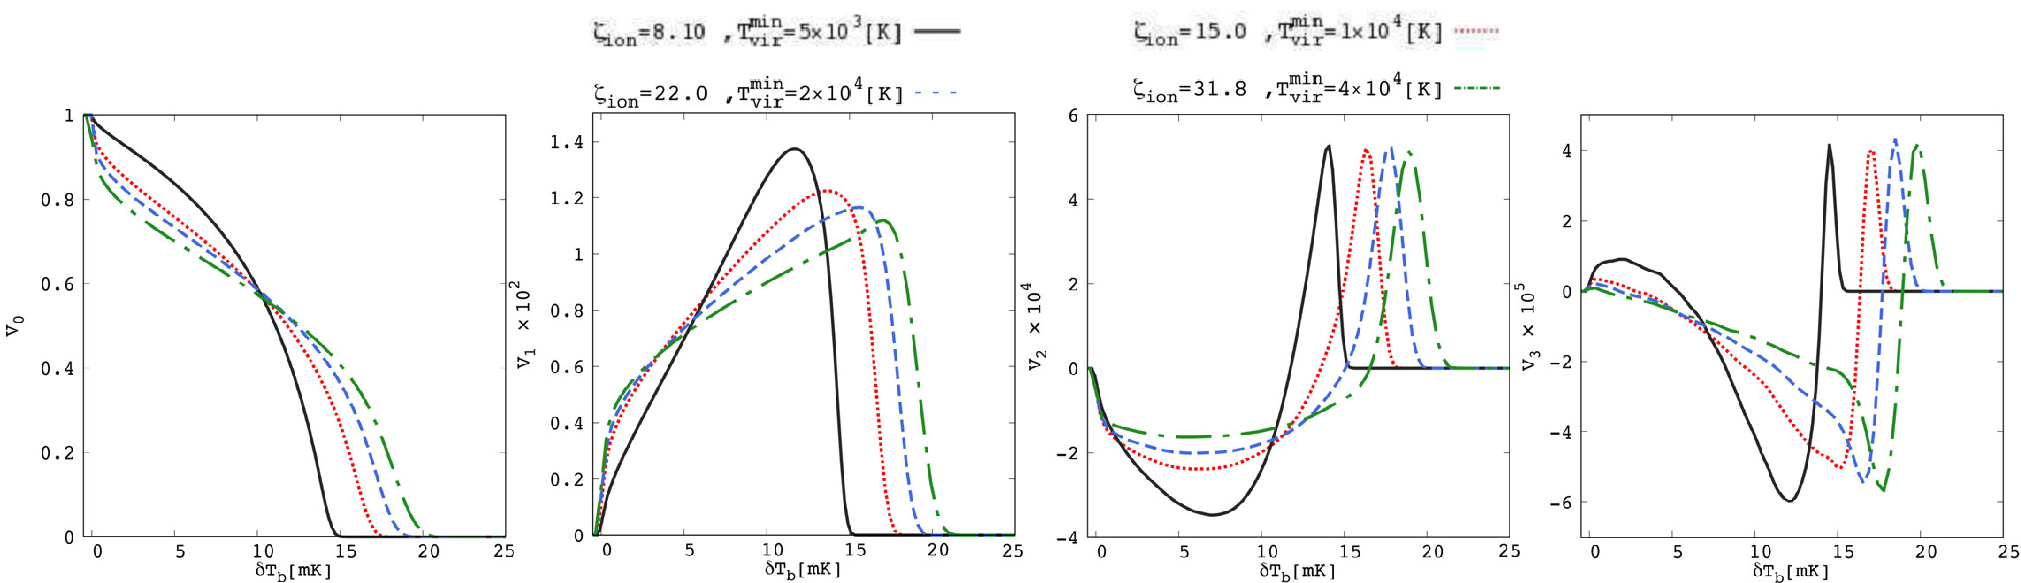
\includegraphics[trim = 0.2cm 1cm 0.2cm 0.2cm, scale = 0.475]{Greig/MFvary}
\end{center}
\caption{The impact of varying the astrophysical parameterisation for a fixed neutral fraction ($x_{H_{\rm \scriptstyle I}}\approx 0.5$) and redshift ($z=8.6$). Consider the impact of varying either the ionising efficiency $\zeta$ or the minimum halo mass for star-forming galaxies, $T_{\rm vir}$ on the four Minkowski functionals. Figure adapted from \cite{Yoshiura:2017}.}
\label{fig:MFs}
\end{figure}

In Figure~\ref{fig:MFs} we show the four Minkowski functionals for the 21-cm brightness temperature when varying the underlying astrophysical processes from \cite{Yoshiura:2017} at a fixed neutral fraction ($x_{H_{\rm \scriptstyle I}}\approx 0.5$) and redshift ($z=8.6$). Here, these authors consider variations in either the ionising efficiency, $\zeta$, or the minimum halo mass hosting star-forming galaxies, $T_{\rm vir}$. Clearly, different reionisation histories are distinguishable by the Minkowski functionals.

\subsubsection{Shape-finders}

An extension to Minkowski functionals, shape-finders ({\color{red} need citations to the method}) are a way to characterise the shapes of compact surfaces. Applied to reionisation (\cite{Bag:2018,Bag:2019}), these shape-finders can provide a means to characterise how the ionised regions grow. For example, they are useful in being able to distinguish between whether the topology is planar or filamentary. Shapefinders are derived directly from the Minkowski functionals via:
\begin{eqnarray}
{\rm Thickness}: T = \frac{3V_{0}}{V_{1}} \\
{\rm Breadth}: B = \frac{V_{1}}{V_{2}} \\
{\rm Length}: L =  \frac{V_{3}}{4\pi}.
\end{eqnarray}
These shape-finders are interpreted as providing the three principle axes of a physical object. The morphology of the ionised region can then be defined by either the planarity or its filamentarity:
\begin{eqnarray}
{\rm Planarity}: P = \frac{B - T}{B + T} \\
{\rm Filamentarity}: F = \frac{L - B}{L+B},
\end{eqnarray}
where $P\gg F$ corresponds to planar objects (i.e. sheets) while the opposite $F\gg P$ corresponds to a filament.

During the reionisation epoch, percolation theory shows that a single infinitely large, multiply connected ionised region will rapidly form ({\color{red} add citations}). When describing the largest singly connected ionised region, \cite{Bag:2018,Bag:2019} find that both $T$ and $B$ evolve slowly whereas $L$ increases rapidly. Thus, this large ionised region grows only along its `length' implying a highly filamentary structure.

\subsubsection{Persistent homology theory}

Homology characterises the topology of the ionisation bubble network into its fundamental components: ionised regions, tunnels (enclosed neutral filaments) and cavities (patches of neutral hydrogen). The persistence then quantifies the significance of the feature, for example its lifetime, by computing a birth and death date for an object.  Thus far, it has only been applied to the ionisation field (\cite{Elbers:2019}). These ionised regions ($\beta_{0}$), tunnels ($\beta_{1}$) and cavities ($\beta_{2}$) can be described by the so-called Betti numbers, which contain the total number of each. These can be related to the earlier Euler characteristic via, $\chi = \beta_{0} - \beta_{1} + \beta_{2}$. By breaking the Euler characteristic into the constituent components and tracking their individual growth reveals additional information on the topology, thus it is a more generalised method than either the genus of the Minkowski functionals.

\subsubsection{Fractal dimensions}

An alternative to classifying the ionised (neutral) regions embedded in the 21-cm signal is through a fractal dimensions analysis. Applied to reionisation (\cite{Bandyopadhyay:2017}), this provides a direct means to quantify the deviation away from a homogenous distribution, as well as the degree of clustering and lacunarity (a measure of the size of the ionised regions). The fractal dimension, $D_{q}$, also known as the Minkowski-Bouligand dimension, is a measure of how complicated the topology of the field in question is. A homogeneous distribution in three dimensions has a $D_{q}=3$. \cite{Bandyopadhyay:2017} show that the topology of reionisation exhibits a significant multi-fractal behaviour. These authors find that the fractal dimension is relatively insensitive to the minimum halo mass of the star-forming galaxies, however it was sensitive to the mass averaged ionisation fraction. Thus, the correlation dimension can be useful for constraining the global neutral fraction. Additionally, it is a strong discriminant of models of outside-in and inside-out reionisation.

\subsubsection{Contour Minkowski tensor}

In \cite{Kapahtia:2018,Kapahtia:2019}, these authors introduced the rank-2 contour Minkowski tensor ({\color{red} add citations}) in two-dimensions which can probe both the length and time scales of the ionised regions during reionisation. The Minkowski tensors are a generalisation of the scalar Minkowski functionals. The contour Minkowski tensor provides information on both the alignment of structures in two dimensions and their anisotropy. Since the ionised regions are not perfectly spherical, their shape anisotropy can be explored by the ratio of the two eigenvalues of the contour Minkowski tensor while the amplitude of the eigenvalues describes their size.

In this analysis, the number of connected regions and holes (e.g. the Betti numbers) given a specific threshold value are tracked. In addition, a characteristic radius of the structures and their shape anisotropy can be determined. For a description of the evolution of $\delta T_{\rm b}$, we refer the reader to \cite{Kapahtia:2019}, ignoring it here owing to its complexity due to the definition of the connected regions and holes as a function of the threshold value as the 21-cm signal transitions transition from hot/cold regions in the heating epoch to neutral/ionised regions during reionisation ({\color{red} would require several figures and long descriptions. Don't think thats required here (hopefully not)}). However, we emphasise that these authors explored varying the minimum mass hosting star-forming haloes and clearly show that different astrophysical parameters can be distinguishable.

\subsection{Bubble size distributions}

Throughout reionisation and the cosmic dawn, the morphology of the 21-cm signal is driven by processes that embed a morphological signature on the 21-cm signal. For example the ionised H$_{\rm \scriptsize II}$ regions or the hot/cold spots in the 21-cm brightness temperature during the heating epoch. Quite simply, if we could measure the distribution of these `bubbles' and how they evolve over cosmic time we would have a strong discriminant of the populations of sources responsible for the heating and ionisation of the IGM and also the spectrum of their emitted radiation. Effectively, this would behave as a statistical distribution function (number of bubbles given a physical scale) analogous to a halo mass function.

However, the bubbles do not remain isolated, very quickly overlapping into increasingly large and topologically complex structures. Thus, there is no unique way to characterise these bubbles. Nevertheless several methods have been explored in order to be able to construct a probabilistic distribution of the bubble sizes.

The simplest approach is to perform a friends-of-friends approach ({\color{red} add citations here}), which simply connects all cells above (below) a threshold value. However, very rapidly a single large ionised structure exists which fills most of the volume with only a small fraction of isolated regions remaining. The relative volume of this large ionised region and the distribution of the smaller regions can still differentiate reionisation morphologies, however there is less statistical weight.

An alternative approach is to place a sphere on every pixel, averaging out the signal across increasingly larger spheres until a radius is found where the average signal is above the threshold value ({\color{red} add citations here}). While this generates a more statistical meaningful distribution of bubbles, these sizes tend to overestimate the size of the topological feature of interest due to the assumed spherical symmetry.

Recently, more statistically robust methods have been introduced to measure the bubble size distributions. First of these is the mean free path method, which uses a Monte Carlo approach by considering a large number of random positions and determining the distance to the edge of the bubble from different random directions ({\color{red}} add citations here). This results in an unbiased estimator of the bubble size distribution. Next, adapted from the cosmological search for voids, the Watershed ({\color{red} add citations here}) method has been explored. This is a well known two-dimensional image segmentation algorithm creating contours of constant value (i.e. $\delta T_{b}$) which are treated as levels of a tomographic map. These are then `flooded' to obtain unique locations for the minima (e.g. ionised regions).

Remaining in the image processing regime, ({\color{red} add citations here}) introduced the superpixels method. This uses a region based method to identify regions of complex shapes (i.e. ionised regions) segmenting these regions into smaller segments called superpixels. The bubble size distribution is then obtained by averaging the value of the 21-cm brightness temperature within each segment ({\color{red} search for specific details on how this becomes a bubble distribution}).

Granulometry


\subsection{Individual bubbles}

Images will provide a direct tangible link to the process of reionisation. Revealing exactly where ionising bubbles are, and thus where to look for the sources responsible for the bubble creation. 

However, bubble identification will become rather problematic, as it is the differential brightness that is observed, not the raw brightness temperature. Need smart/sophisticated approaches to search and characterise the signal.

Look at individual regions of interest, i.e. around a bright QSO or large number of galaxies. 

Matched filters etc., are useful for finding/detecting isolated bubbles

\subsection{Stacked images}

May be difficult to detect individual objects, instead, one could stack 21cm spectra centred on known galaxies. See Paul Geil's paper.

Border's on potential discussions of synergies. Requires known locations of ionising sources with precise redshifts and positions of the sky. JWST/WFIRST. Is there 

\subsection{Other statistics}

Are there other statistics that I have overlooked/forgotten. Need to do a search of the literature to ensure I have covered everything.

\section{Efficient methods to model/simulate the 21cm signal}

Ideally we want to use the largest, most physically accurate simulations to match the observed 21cm signal. However, this is not practical. Instead, we must come up with methods to compensate accuracy for efficiency.\\
\\
Originally I envisaged this section to go as follows
\begin{itemize}
\item Discuss briefly that numerical simulations are great but too computationally expensive
\item Highlight semi-numerical/analytic simulations as fitting the bill by being faster etc.
\item Then discuss alternatives (i.e. emulators).
\end{itemize}
This will need to be re-worked given Jordan's plan to discuss this. I haven't yet thought of a logical plan to motivate this. I guess one way would be to concatenate it into just a simulation section and briefly summarise what was discussed in Jordan's chapter (which is a couple of chapters ago, so might be appropriate to do so). It's less obvious to move into discussing emulators in the absence of motivating the need for them by highlighting the complications of simulations in general.

\subsection{Numerical simulations}

Ideally, use large, numerical simulations to make a realisation which matches observation. Want to include as much physics as possible into these simulations. Doing so, comes at a serious cost. Simulating the 21cm signal is complicated! Brief summary on the required dynamic range. Briefly highlight the expensive nature of these simulations, Hydrodynamics, radiative transfer etc. Quickly becomes computationally prohibitive to run more than a couple of realisations. \textbf{Jordan's section (Modelling Tools) will likely cover most if not all of this}.

\subsection{Semi-numerical/analytic models of the 21cm signal}

Enter semi-numerical approaches, which broadly encapsulate the global average quantities of reionisation and the cosmic dawn and reproduce morphologically similar realisations of the 3D structure. The advantage here is that the computational costs are drastically reduced (orders of magnitude less). \textbf{Jordan's section (Modelling Tools) will likely cover most if not all of this}.

\subsection{Intelligent sampling of the parameter space}

Running simulations to span all of the allowed parameter space may be too computationally intensive. However, perhaps we can make intelligent assumptions/guesses about how many simulations to run, and on a specific area of physics to focus on. Some of the concepts here may overlap slightly with the Emulator section below. This sampling was discussed in one of Benoit's recent papers.

\subsection{Emulators}

An alternative to directly running a simulation to estimate some astrophysical statistic/model, one can instead construct a function which estimates what the statistical signal should be, given some astrophysical or cosmological parameter set. This is what is referred to as an emulator. Using simulations, a generator function is constructed which can approximate the statistics of the signal. Results in multiple orders of magnitude improvement in computational speed as no new simulations are required. However, it can only approximate statistics, it does not generate 3D simulations. 

Developing an emulator benefits from efficient parameter space approaches, as it minimises the size of the database required to construct the emulator. There are a variety of approaches to consider when attempting to minimise the sampling of the astrophysical parameter space. For example Latine-Hypercube, Gaussian processes... Can briefly discuss each method, and a few recent papers that explore methods to do this

There are numerous machine learning approaches to construct an emulator.

Discuss Nick Kern's of 21cmFAST and Cohen's global signal one of Anastasia's code.

Highlight and discuss Chardin et al. (2019). Emulation of reionisation simulations (construction of treion maps given source lists). arxiv:1905.06958

\subsection{Characterising our ignorance}

We are fully aware that semi-numerical approaches are inaccurate at 10s of per cent level. Additionally, they oversimplify/completely ignore the underlying astrophysical properties. However, if the global quantities (observables such as luminosity functions etc.) can still be reproduced within agreement, we can develop an understanding of how one might map from a semi-numerical simulation, to a more realistic simulation. Basically, tell the large, computationally expensive simulation where exactly to look in the region of parameter space.

Using summary statistics and globally average observables, we can develop a means to calibrate one simulation to mimic the outputs of another. In other words, develop a bias or functional form to smooth out uncertainties from one simulation to mimic the results of a more detailed simulation.

Describe ongoing attempts to quantify this. i.e. use luminosity functions to calibrate simulations, apply redshift corrections to deal with photon non-conservation etc.

These correction factors etc., will be crucial for inferring astrophysics and cosmology from the 21cm signal


\section{Inference methods for 21cm}

Having discussed methods to model/simulate the 21cm signal, now need to shift focus to methods to infer information about the astrophysics/cosmology from the 21cm signal.

\subsection{Fisher Matrices}

Simplest method, which takes derivatives with respect to model parameters of a functional form (i.e. a 21cm statistical signal) to infer parameter constraints. Effectively, exploits how sensitive the 21cm signal is to specific parameters. Limiting assumption include Gaussianity etc.

Successfully used for cosmology

\subsection{Bayesian MCMC}

Significantly more robust method to parameter inference. Outline Bayes' theorem. Highlight that this basically boils down to exploring by random walks, using a likelihood function and priors to accept/penalise regions of parameter space. Very useful for recovering constraints. Again, successfully used in Cosmology etc.

Describe its use in the context of 21cm. Introduce 21CMMC, and a couple of other codes that use MCMC (Sultan's simfast21, Jordan's global signal, Geraint's MCMC, Simon's Mhysa). Highlight that 21CMMC is the only direct MCMC. Emphasise that techniques such as emulators can be coupled with MCMC to improve overall computational efficiency at the cost of some further inaccuracies.

Don't forget the Bernardi and Zwart papers.

\subsection{Nested sampling and model inference}

We have a wide variety of simulations, each with their own strength's and weaknesses. In principle, various models/simulations/physical prescriptions can be discriminated against using model selection or inference. Related to MCMC, nested sampling can focus on model selection rather than simply astrophysical recovery. Can refer to Tom Binnie's recent paper.

\subsection{Neural Networks}

Instead of using MCMC to recover parameters from statistics, we can use the full 2/3D images of the 21cm signal with neural networks. One can construct a database of simulations and extract the 21cm signal to construct a neural network. This network can then learn an large number of properties, i.e. how changes in the topology are affected by astrophysical parameters etc. Using this technique one can directly convert from an observed 2D image to the underlying astrophysics. Like emulators, the application of the network is extremely quick. Downsides are parameter errors etc. and in some sense physical intuition. It tells you an answer, but not why.

Simulated images of the 21cm signal have already been used to infer astrophysical and cosmological constraints. For example with convolutional networks (e.g Nicolas or Paul La Plante). Discuss other machine learning approaches.



\iffalse

Lorem ipsum dolor sit amet, consectetur adipiscing elit. Duis eu egestas erat. Maecenas tincidunt lacinia tincidunt. Mauris id lectus nec neque feugiat condimentum vitae at diam. In vel orci nunc, non commodo mauris. Vivamus ipsum enim, vulputate quis pharetra non, molestie quis felis. Vivamus porttitor placerat turpis at accumsan. Nunc tortor velit, faucibus a rhoncus nec, blandit non elit. Nam consectetur lectus eu nisi blandit dapibus rhoncus dui tempus. Mauris fermentum dolor vel ipsum vulputate sit amet ultricies tortor lacinia. Donec ut nibh erat. Morbi nec mi ante. Integer nec vestibulum diam. Donec tincidunt pellentesque quam, ut interdum mauris venenatis condimentum. Nam condimentum, augue in aliquet gravida, neque dui elementum eros, id semper eros purus sed felis. Curabitur in justo sit amet sapien ultrices hendrerit at quis nibh. Quisque iaculis pulvinar tincidunt. 
\begin{eqnarray}
C(12) &= &\left[\overrightarrow{\pi}\cdot\overrightarrow{\phi}(x+r)\right] \nonumber \\ 
&\approx& 1-\mathrm{const}\frac{r^2}{L^2}\int_r^L\frac{x\rmd x}{x^2} + \cdots \nonumber  \\
&\approx& 1-\mathrm{const}\frac{r^2}{L^2}\ln\frac{x\rmd x}{x^2} + \cdots .\label{brokenlongeqn}
\end{eqnarray}

Aenean tellus risus, porta sit amet porta vitae, tincidunt ut felis. Class aptent taciti sociosqu ad litora torquent per conubia nostra, per inceptos himenaeos. Vestibulum ante ipsum primis in faucibus orci luctus et ultrices posuere cubilia Curae; Phasellus pulvinar placerat velit auctor egestas. Vivamus euismod fringilla tincidunt. Sed ut magna felis, id sollicitudin nunc. Quisque a dui eu erat consectetur egestas a quis justo. Aenean euismod congue diam, vel posuere urna fermentum sit amet. Lorem ipsum dolor sit amet, consectetur adipiscing elit. Mauris faucibus lacus eget est mollis auctor. Donec at nibh ligula, et posuere massa. Phasellus quis leo diam \cite{diamantaras1996pcn}.
Donec aliquam blandit risus, eu venenatis ante euismod eu. Curabitur cursus justo id arcu condimentum feugiat. Integer sapien urna, vulputate et adipiscing nec, convallis et justo. Suspendisse in ipsum at felis ornare interdum \cite{tulone2006pts},

\begin{figure}[]
\begin{center}
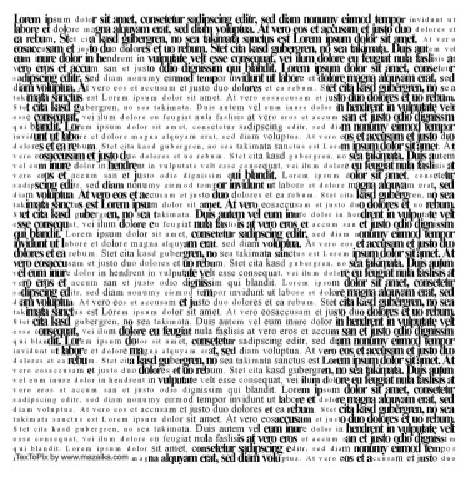
\includegraphics[width=0.5\textwidth]{Greig/01x01-eps-converted-to}
\end{center}
\caption{This is figure 1 in chapter 1.}
\end{figure}

\paragraph{Cras adipiscing} sagittis nunc vel luctus. Suspendisse volutpat augue quis erat semper consequat dignissim tellus euismod. Morbi hendrerit, tellus id aliquam iaculis, nibh leo tincidunt eros, vitae varius ligula felis in mi.

\begin{table}
\caption{Greek Letters.}
\begin{center}
\begin{tabular}{llllllll}
\hline
$\alpha $  & $ \beta $  & $ \gamma $  & $ \delta $  & $ \epsilon $  & $ \varepsilon $  & $ \zeta $  & $ \eta $ \\
 $ \theta $  &  $ \vartheta $  &  $ \gamma $  &  $ \kappa $  &  $ \lambda $  &  $ \mu $  &  $ \nu $  &  $ \xi $ \\
 $ o $  &  $ \pi $  &  $ \varpi $  &  $ \rho $  &  $ \varrho $  &  $ \sigma $  &  $ \varsigma $  &  $$ \\
 $ \tau $  &  $ \upsilon $  &  $ \phi$ &  $ \varphi $  &  $ \chi $  &  $ \psi $  &  $ \omega$  &  $ $ \\
 &  &  &  &  &  &  & \\
$ \Gamma $  & $ \Delta $  & $ \Theta $  &  $ \Lambda $  &  $ \Xi $  &  $ \Pi $  &  $ \Sigma $  & $ \Upsilon $ \\
 $ \Phi$ &  $ \Psi $  &  $ \Omega $  &  &  &  &  &\\
\hline
\end{tabular}
\end{center}\end{table}

\begin{figure}[]
\begin{center}
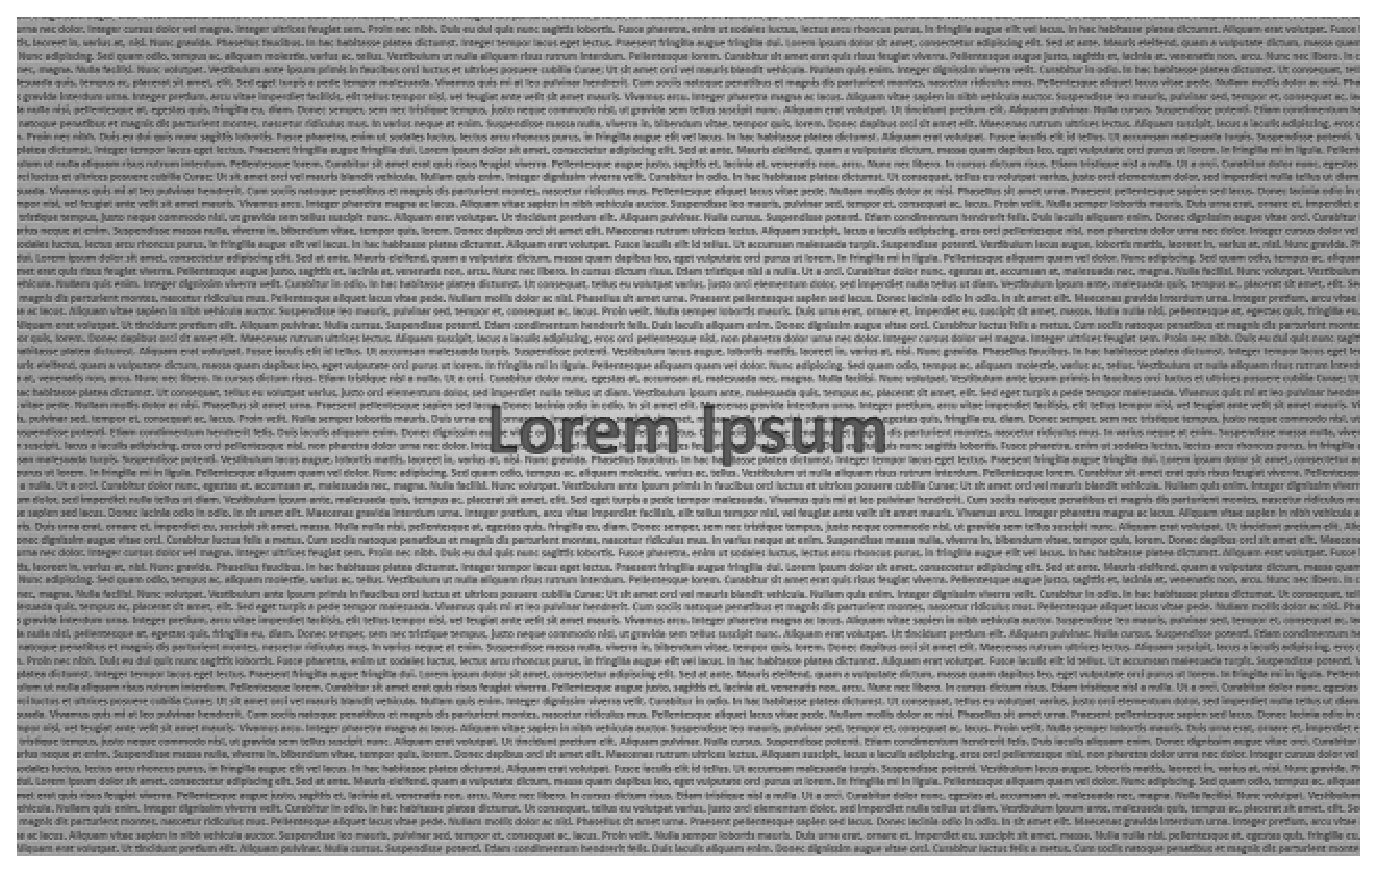
\includegraphics[width=0.6\textwidth]{Greig/01x02}
\end{center}
\caption{This is figure 2 in chapter 1.}
\end{figure}

\fi

\bibliographystyle{plain}
\bibliography{Greig/References}


